\documentclass[]{final_report}
\usepackage{graphicx}
\usepackage{hyperref}
\usepackage[dvipsnames]{xcolor}
\usepackage{verbatimbox}
\usepackage{multirow}
\usepackage{tabularx,booktabs}
\usepackage{mathtools, nccmath}
\usepackage{mathtools}
\newcolumntype{Y}{>{\centering\arraybackslash}X}
\usepackage[skip=2pt,font=normalsize]{subcaption}
\usepackage[skip=2pt,font=normalsize]{caption}
\usepackage{enumitem}
\usepackage{fancyvrb}
\usepackage{xcolor}
\usepackage{amsmath}
\usepackage{rotating}
\usepackage{amssymb}

\newcommand{\numberset}[1]{\mathbb{#1}} 
\newcommand{\nat}{\numberset{N}}
\setlist{nosep}
\usepackage{tikz} 
\usetikzlibrary{positioning}
\usepackage{xfrac}
\usepackage{array}
\newcolumntype{P}[1]{>{\centering\arraybackslash}p{#1}}
\newcolumntype{M}[1]{>{\centering\arraybackslash}m{#1}}
\renewcommand{\arraystretch}{2}
\usepackage[toc,titletoc,title]{appendix}

\usepackage{caption,tikz}
\usepackage{subcaption}


\DeclareCaptionFormat{suboverlay}{\gdef\subcapoverlay{\colorbox{black!30}{(\thesubfigure) #3\par}}}
\DeclareCaptionStyle{suboverlay}{format=suboverlay}

\DeclareCaptionFormat{suboverlayright}{\gdef\subcapoverlay{\colorbox{black!30}{(\thesubfigure) #3\par}}}
\DeclareCaptionStyle{suboverlayright}{format=suboverlayright}


%TC:group tabular 1 1
%%%%%%%%%%%%%%%%%%%%%%
%%% Input project details
\def\studentname{Natalia Kenrick}
\def\reportyear{2022/23}
\def\projecttitle{Single-Agent and Multi-Agent Search in Maze Games}
\def\supervisorname{Farid Shahandeh}
\def\degree{BSc Computer Science (Artificial Intelligence)}
\def\fullOrHalfUnit{Full Unit} % indicate if you are doing the project as a Full Unit or Half Unit
\def\finalOrInterim{Final Report} % indicate if this document is your Final Report or Interim Report

\begin{document}

\maketitle

%%%%%%%%%%%%%%%%%%%%%%
%%% Declaration

\chapter*{Declaration}

This report has been prepared on the basis of my own work. Where other published and unpublished source materials have been used, these have been acknowledged.

\vskip3em

Word Count:

\vskip3em

Student Name: \studentname

\vskip3em

Date of Submission: 

\vskip3em

Signature:\par\medskip
\includegraphics[height=2\baselineskip]{Dissertation/Pictures/signature.pdf}\par 

\newpage

%%%%%%%%%%%%%%%%%%%%%%
%%% Table of Contents
\tableofcontents\pdfbookmark[0]{Table of Contents}{toc}\newpage

%%%%%%%%%%%%%%%%%%%%%%
%%% Your Abstract here

\begin{abstract}
The aim of the project is to implement general search algorithms in single and multi-agent environments in order to find the optimal route through a maze and to complete some goal. By designing and implementing agents with different tasks, each will need to find efficient ways through the maze in order to complete their goal.

This project is intriguing because it shows how we can use autonomous agents to complete some task without user input. This is especially interesting in a multi-agent scenario where agents can communicate and help each other to reach their goals. 

In order to implement the search algorithms in our maze, we will model the maze as a search problem. By using simple uninformed search algorithms such as depth-first search and breadth-first search, we can find a specific location in a maze. Later, we can introduce a cost function to our search to find the shortest distance. We can also apply more complex search algorithms, such as the A* algorithm, which uses a heuristic in order to better inform our agent of its surroundings. 

We will also take a look at adversarial searches, a game theory approach to searching. We use these in a scenario where our agents do not work together but are adversaries trying to win a game. This will be a multi-agent scenario where we can observe the actions that our agents take.

Lastly, we will touch on reinforcement learning and see how we can write our agent in a way that it can learn from its actions and improve over time.

By combining different search algorithms and techniques, we can produce the most optimal outcome for our goal.
\end{abstract}
\newpage

\chapter*{Project Specification}
\addcontentsline{toc}{chapter}{Project Specification}

%TC:ignore
\begin{minipage}{\textwidth}
\textbf{Aims:} The goal of this project is to implement general search algorithms and apply them to single-agent and multi-agent scenarios in maze games (e.g. Pac-Man).

\textbf{Background:} Maze games are a video game genre in which the entire playing field is a maze. Usually, the player needs to navigate the maze to collect items and also performs other actions (e.g. escape monsters and outrace an opponent) within a time limit. The most popular example is Pac-Man by Namco (1980), but many other maze games exist. You will model a maze game as a search problem and then design and implement agents that inhabit the maze. The agents will find efficient paths through the maze world, to reach a particular location, to collect food and to combat opponents.

\textbf{Early Deliverables}

\begin{enumerate}
    \item Given a maze game of your interest (e.g. Pac-Man), design and implement a simple graphical visualisation for it.
    \item Consider an agent inhabiting the maze world. Model the agent's navigation task as a search problem. Implement a graph search version of depth-first search and breadth-first search to reach a specific location in the maze. Run experiments with three different size maze: small, medium and large. Visualise the agent following the plan step-by-step.
    \item Now change the cost function in such a way that traversing some areas is more expensive than traversing other areas (e.g. Pac-Man: you can charge more for dangerous steps in areas close to the ghosts). Implement the uniform-cost graph search algorithm to reach a specific location in the maze. Run experiments with three different size maze: small, medium and large. Visualise the agent following the plan step-by-step.
\end{enumerate}

\textbf{Final Deliverables}

\begin{enumerate}
    \item Implement the algorithm A* to find the shortest path through the maze that touches all four corners. Use two different, consistent heuristic functions. Run experiments with three different size maze: small, medium and large. Visualise the agent following the plan step-by-step.
    \item Assume each cell in the maze has an item to collect. Formulate a search problem for collecting all items (e.g. in Pac-Man: eating all the food) and implement A* to do that in as few steps as possible. Also implement a greedy search and compare the results of the two algorithms in three different size maze: small, medium and large. Visualise the actions of the agent.
    \item Now assume that you have additional agents in your maze, one is the main player and the other are the opponents (e.g. Pac-Man and the ghosts). Model this new problem and implement the player as a reflex agent that tries to visits all cells avoiding the opponents.
    \item Implement an adversarial Minmax search agent for each agent; start with the player and one opponent and then increase the number of opponents. You need to write an evaluation function that evaluates states. Run experiments with three different size maze: small, medium and large. Visualise the actions of the agents.
    \item Design and implement a new agent that uses Alpha-beta pruning to more efficiently explore the minimax tree. Run experiments with three different size maze: small, medium and large. Visualise the actions of the agents.
    \item Design and implement an Expectimax agent to model the probabilistic behaviour of an agents who makes suboptimal choices. Run experiments with three different size maze: small, medium and large. Visualise the actions of the agents.
\end{enumerate}

\textbf{Suggested Extensions}
\begin{itemize}
    \item Use value iteration and Q-learning to underpin the behaviour of the player.
\end{itemize}
\end{minipage}
%TC:endignore

%%%%%%%%%%%%%%%%%%%%%%
%%% Introduction
\chapter{Introduction}

\section{Idea}

When developing large systems with many smaller sub-problems, sometimes using functional programming, or even object-oriented programming can be difficult. Multi-agent systems can be incredibly useful when used to decompose a difficult problem into lots of small sub-problems. 

A multi-agent system is a society of distributed autonomous, cooperative entities\cite{leitao2013multi} in which each agent has its own goal, knowledge base, and agent program (further details in section \ref{Agents and Environments}).

An example of how we can implement a multi-agent system could be planning a traffic route for hundreds of self-driving cars. This problem would be nearly impossible if executed functionally. However, if we were to approach this problem in the multi-agent paradigm, we can abstract the problem into manageable pieces. If we turn each car in this instance into an agent, with its own set of instructions to follow, then suddenly we aren't dealing with hundreds of cars, we can focus on how to make a single agent get to its destination, and how it should interact with others as it does. 

One real-world example of how multi-agent systems can be implemented is SARDINE (System for Airline Reservations Demonstrating the Integration of Negotiation and Evaluation). SARDINE uses agents to coordinate the preferences and interests of a buyer. The buyer agent takes this information and correlates these to available flights from a reservation database. The user then informers the buyer agent on how much it should bid. The airline agents accept the ticket bids from the buyer agent. Finally, the airline agents consider individual bids based on flight yield management techniques and specific buyer information\cite{oprea2004applications}.

Search algorithms are very useful when it comes to pathfinding. We will be implementing a commonly used informed search, A* in order to find our goal. One example of how we could potentially apply this algorithm to a real-life scenario is by using Unmanned Aerial Vehicles (UAV). As suggested by their name, these vehicles do not have a pilot. It uses other means to pilot itself such as ground crew and GPS. Although there are satellites that they can use, they usually use a fixed-ground wireless receiver. This however means that the telemetry (automatic measurement and wireless transmission of data from remote sources) of the UAV is limited by the transmission distance of the transceiver. To solve this, UAVs can use pathfinding for civil UAVs using 3g base stations \cite{6998482}.

We want to use agents as they are extremely useful tools that can be used in many different types of applications. They scale a lot better than objects, which do not have autonomy over their actions (Kostas Stathis 2022). They can be thought of as active objects that have initiative. They require less organisation on implementation when compared to objects as they can organise themselves. Let's imagine we have many agents completing some task, if one fails, the impact on the system as a whole may be minimal, but if an object fails an exception is raised.\cite{odell2002objects}. Often, they are implemented to act as an extension of the user. By this, we mean that they provide some service to the user that would otherwise prove time-consuming if completed themselves e.g. browsing the internet for specific files. We can use an agent to do this task; It will work continuously without getting tired or distracted and can be programmed to only gather the information that is known to be useful for the user\cite{jennings1996software}.  
 
\section{Aims and motivations}

The aim of this project is to show how we can use agents to solve problems autonomously. More specifically, we will be demonstrating how agents can navigate their way through a maze using search algorithms, in both single and multi-agent scenarios. By visualising the routes they take we can display how they change their behaviour based on the goal they wish to achieve. 

We use search algorithms to find the shortest path. They can be used in many ways, including complex issues such as optimal energy-efficient path planning for an unmanned air vehicle\cite{debnath2019review}. We aim to implement two forms of search algorithms, uninformed and informed. Informed searches are more efficient than uninformed searches as they have more information about the problem itself and are able to use methods such as heuristics functions to work out the optimal path.

We also hope to show how other methods of agent programming, such as reinforcement learning and adversarial searches, can be implemented and trained to complete some goals as optimally as possible.

By the end of this project, we hope to showcase how the use of intelligent agents can be used to automate tasks by displaying how their decision-making movements occur in a game-like scenario. 
\newpage

\section{Background}
\subsection{Agents and Environments}\label{Agents and Environments}

One of our main focuses in this report is about agents, so first, let's understand what they are and how they work. We will look at agents as a whole, the agent types and how we use them, and identify environments and how agents interact with them. 

An agent is defined as anything that can perceive its environment through sensors and can complete some autonomous action through actuators. For example, as humans, we have eyes, ears touch etc which allow us to sense and see our environment, and we act with our legs, hands, voice and many more. An agent could be robotic, using light sensors, heat sensors and more to perceive its environment and could have a range of actuators such as robotic arms, wheels etc. A software agent can use sensory inputs such as keystrokes and act upon an environment by displaying them on the screen.

An agent needs to know how to map percepts to an action, to do this they use what is called an agent function; It decides what action the agent should perform given the current percepts. An agent is comprised of two properties, an agent function and an agent program. The agent program is the internal, executable implementation of the agent function. 

Agents are not automatically considered intelligent, they must conform to certain characteristics. Wooldridge\cite{WooldridgeMichael2009AitM}, defines an agent to be intelligent if it has the following characteristics: reactivity, pro-activeness and social ability. What we mean by this is that an agent is able to react to changes in its environment in a timely fashion, make decisions based on their goal, and can communicate with other agents. These characteristics of intelligence become crucial when working in multi-agent scenarios. A multi-agent system uses many intelligent agents of the same or different types in order to achieve some task/goal. Often, scenarios involve working together to complete a combined goal, but as a result, agents have their own tasks. Agents need to be able to communicate and react to other agents, whilst making sure to stay focused on their tasks. An example of intelligent agents working together is the well know scenario Vacuum World. Let's say we have two agents, Orange and White. Their combined goal is to make sure there is no dirt in the grid, their individual goal is to clean up dirt of their own colour. In this scenario, the white agent can communicate to the orange agent that it has seen orange dirt, and vice versa (social ability). The orange agent can react to this message by heading toward the known dirt location (reactivity and pro-activeness).

An agent in a multi-agent scenario would have different characteristics from an agent in a single-agent scenario. An agent can have certain characteristics that make it suitable for different goals. For example, some agents have a knowledge base (a set of facts/beliefs about the environment) which means they can make informed decisions. Let's have a look at some agents we will be using and how they work.

A \textbf{goal-based agent's} decisions are based on whatever gets it closer to its goal. At each state, it needs some sort of information to do with the goal in order to pick the action that is the most desirable. We will use a type of goal-based agent called a problem-solving agent. This problem-solving agent will be used when showcasing search algorithms. This type of agent is used because it doesn't care about the internal structure of the states - only how far away they are. A search algorithm can take the problem as input and return an action sequence for the agent to then carry out. By doing this, the agent is not taking into account new precepts, therefore best used in a static environment where nothing will change except by actions of the agent  itself\cite{russell2016artificial}. We will see more about agent environments later. 

A \textbf{simple reflex agent} is the most simple agent to use. They choose their actions based on their current percept, they do not have a history of past actions or percepts. A simple reflex agent is only able to perform actions in a fully observable environment. This is because they work by reacting to their current percepts, without them they do nothing. They are most useful in small environments performing basic experiments (Kostas Stathis 2022).

\textbf{Reinforcement Learning Agents} are more simple than they sound. They use a reward function as well as other RL features in order to inform their decision-making. We will explain this in a lot more detail in section \ref{Reinforcement Learning}, but the basic idea is they receive feedback in the form of rewards and they must learn how to maximise them.

We will see in section \ref{unininformed search implementation} how these agents work when implemented to complete some tasks in a maze environment. 

To be able to use an agent, it needs to be situated in an environment. When specifying the agent environment, we can use the PEAS (Performance, Environment, Actuators, Sensors) description. Let's look at an example, Vacuum World. We gave a brief description already, but let's have a closer look. Agents are situated in an $n$ x $n$ grid, They are able to move around the grid in order to clean up dirt of their own colour. They may communicate with other agents, and can only see 6 surrounding squares. In this example we have:
\begin{itemize}
    \item \textbf{Performance measure:} Clean all dirt in the grid.
    \item \textbf{Environment:} A $n$ x $n$ grid in which our agent can move in any direction freely - except in the case where the agent would leave the grid. Clean squares stay clean and an agent can only clean a square they are currently on. Two agents cannot be on the same square at the same time and cannot clean dirt that is not their own colour.
    \item \textbf{Actuators:} An agent can move forward or turn in a different direction. They can clean. They can do some form of communication.
    \item \textbf{Sensors:} An agent can see 6 surrounding squares - two by their side, one directly in front of them, one to their front-left and one to their right,  as well as the square they are currently on. They cannot see behind them. They are able to receive messages from other agents.
\end{itemize}

This is helpful in breaking down the problem, but still doesn't give us enough detail; we need to specify the properties of the environment. Our agent in Vacuum World is only able to see a small portion of the environment it is in. This means it is \textbf{partially observable}. The are many properties that our environments may have.

\textbf{Fully observable vs partially observable} - Can our agents get full and correct information about the environment? In the case of Vacuum World, we cannot get a full, correct representation of the world therefore it is \textbf{partially observable}.

\textbf{Deterministic vs stochastic} - Does it hold that each action has only 1 known outcome (guaranteed and uniquely defined)? In this example all action outcomes are known - there is no uncertainty, therefore it is \textbf{deterministic}.

\textbf{Episodic vs sequential} - Does the agent's action depend on the previous? In episodic, an agent receives a percept and performs some action - the next episode does not depend on the actions taken in the previous episode. Our example is \textbf{sequential} because the decision the agent makes depends on the last state e.g which dirt to clean next.

\textbf{Static vs dynamic} - Does the environment change out of our agent's control? In Vacuum World we can have many agents - each moving and changing the environment, this means our environment is \textbf{dynamic}.

\textbf{Discrete vs continuous} - Are our actions and percepts fixed and finite? Our example is \textbf{fixed}, there is a finite number of states the action could be in, a fixed number of actions they could perform as well as precepts they could sense.

\textbf{Single-agent vs multi-agent} - Does our agent's behaviour rely on that of another? This is obvious in the case of Vacuum World, our agent relies on the other agent completing its job in order for the grid to be clear of \textit{all} dirt.

Specifying the task environment and the properties it will have can help us understand how our agent should interact with it. By doing this we have laid out our problem, allowing us to construct our agents as our solution. 

'\subsection{Search Algorithms}\label{Search Algortithms}

The next main component of our project is search algorithms. We will first look at what a search problem is, and then move on to algorithms. We will look at uninformed searches, which do not hold any information about the nature of the problem, only the definition they are given. We will then look at informed searches which can solve the same problems as our uninformed algorithms but are generally more efficient. 

We will need to model the maze as a search problem in order to apply these algorithms. Wolfgang Ertel\cite{Ertel_2011} states that a search problem can be defined by having the following properties:

\begin{itemize}
    \item \textbf{State:} The state of the world the agent is in
    \item \textbf{Start State:} Initial state of agent
    \item \textbf{Goal state:} The goal state of the agent, where it terminates and returns a solution
    \item \textbf{Actions:} The actions our agent can take
    \item \textbf{Solution:} Path taken or to be taken by our agent
    \item \textbf{A cost function:} Cost value of an action (path cost). In the case of no path cost, each action has an equal value
    \item \textbf{State Space:} Set of all states
\end{itemize}

We will use this design when modelling our problem.

\subsubsection{\Large{Uninformed Search}}\label{Uninformed search} 

The first type of search we will look at is an uninformed search (also known as blind search), which does not hold any information about the number of steps to reach the goal. It only considers which path is most promising at a point in time, but not the most optimal\cite{pathak2018comparative}. These searches only know whether or not the current state is or isn't the goal state. They expand every node in a brute-force kind of way. We want our agent to demonstrate how these searches work. To do this our uninformed search algorithms take our agent's problem as an input and return the solution in the form of an action sequence for our agent to then execute. \cite{russell2016artificial}.

\textbf{Breadth-first Search}\label{Breadth-first Search}

A breadth-first search (BFS) is a simple uninformed search that works by expanding all nodes at the same depth level, before moving on to the next. This search uses a first-in-first-out (FIFO) queue when expanding nodes, this is inefficient as goals on the bottom level are expanded last. A BFS does not consider path cost when expanding nodes which means it is best used on a graph with equal or no path costs.


\begin{minipage}[!htp]{0.5\linewidth}
The steps of performing a BFS are:\\
\begin{enumerate}
    \item Add initial state to an explore list \textbf{E}
    \item Take the first item in the list \textbf{X}, add to list of visited states, \textbf{V}
    \item If \textbf{X} is our goal, stop. Else
    \item Find all children of \textbf{X}.
    \item If children of \textbf{X} do not appear in either \textbf{E} or \textbf{V}, add child to end of \textbf{E}
    \item Repeat from step 2 until list \textbf{E} is empty
    \item Return \textbf{V}
\end{enumerate}
\end{minipage}\hfill
\begin{tikzpicture}[baseline=0cm]
  \node (A) {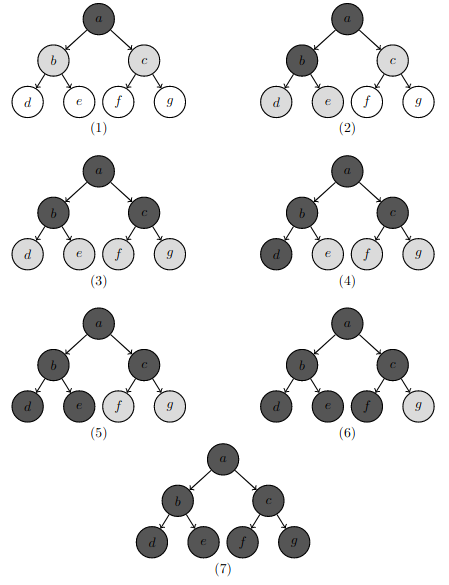
\includegraphics[width=.4\linewidth]{Dissertation/Pictures/BFS.png}};
\end{tikzpicture}


When measuring the efficiency of these algorithms we can look at their time complexity. Time complexity is the computational complexity which describes the time taken for an algorithm to run. For a BFS, this is $O(|V| + |E|)$ where $|V|$ represents the number of vertices and $|E|$ represents the number of edges. However, if we were to be working in a tree of infinite size, the running time can be written as $O(b^d)$. The reason for this is that if we have a tree of infinite size, we do not know the number of edges or vertices per se. $b$ represents the branching factor, the number of children at each node ($b$ = maximum branching value, its the worst case). $d$ represents the depth of the shallowest solution. We can think of this as looking $d$ steps ahead.

\textbf{Depth-First search} 

A depth-first search (DFS) is another example of a simple uninformed search. It expands a node all the way to its deepest child, before returning to the next deepest node and expanding that all the way etc. A depth-first search uses a last-in-first-out (LIFO) queue, opposite to a BFS. This means it's always expanding the deepest unexpanded node. Like a BFS, a DFS does not consider path cost when expanding nodes. We will be using the DFS on a graph structure, meaning there is a finite number of nodes for it to expand; however, let's say we were working on an infinite binary tree, if our goal state is the first node on the right but we expand the left side first, we will never reach our goal as it will keep expanding the deepest node forever. If this was the case, we could use a depth-limited DFS (Depth-limited search) as we will see in section \ref{Depth-limited search}.



\begin{minipage}[!htp]{0.5\linewidth}
Steps for performing a DFS:
\begin{enumerate}
    \item Add initial state to a explore list \textbf{E}
    \item Take the last item in the list \textbf{X}, add to list of visited states, \textbf{V}
    \item If \textbf{X} is our goal, stop. Else
    \item Find all children of \textbf{X}.
    \item If children of \textbf{X} do not appear in either \textbf{E} or \textbf{V}, add child to end of \textbf{E}
    \item Repeat from step 2 until list \textbf{E} is empty
    \item Return \textbf{V}
\end{enumerate}
\end{minipage}\hfill
\begin{tikzpicture}[baseline=0cm]
  \node (A) {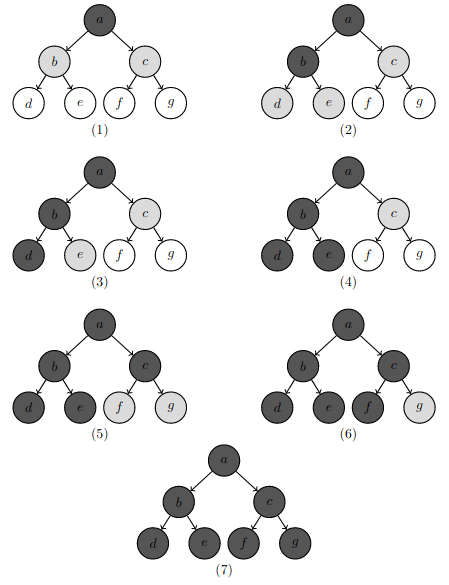
\includegraphics[width=.4\linewidth]{Dissertation/Pictures/DFS.png}};
\end{tikzpicture}

Notice the steps are almost identical to The BFS shown in \ref{Breadth-first Search}, only this time we expand the last item. This can be done recursively, with no significant improvement in running time (but looks nicer, \ref{fig: recursive dfs}). 

\begin{verbbox}
def RecursiveDFS(node, path):
    path.append(node)
    for each child of node:
        if node not in path:
            RecursiveDFS(child, path)
\end{verbbox}
\begin{figure}[ht]
  \centering
  \theverbbox
  \caption{Pseudocode for recursive DFS}
  \label{fig: recursive dfs}
\end{figure}


The running time for a DFS is $O(|V| + |E|)$, the same as a BFS. In the case of an infinite tree, the running time is $O(b^m)$ where $b$ is the branching factor and $m$ is the maximum depth.

\textbf{Depth-limited search} \label{Depth-limited search}

When trying to find a goal in a DFS we want to make sure we are not looking any deeper than we need to. If we know that the goal is within the first \textit{d} levels of our tree/graph then we can set a limit to our DFS. This is called a depth-limited search. A depth-limited search works the same as a DFS but assumes nodes at depth \textit{d} has no children. If we don't know where the goal is, we can perform and \textbf{iterative deepening search}, which increases the depth \textit{d} until we find the goal. The running time is $O(|V| + |E|)$, same as a BFS. In the case of an infinite tree, the running time is $O(b^l)$ where $b$ is the branching factor and $l$ is the depth limit.

\textbf{Uniform-cost search}

As stated earlier in the chapter, A BFS performs best on a graph with equal or no path cost. But when we do have a path cost, BFS is significantly less optimal. To build on this idea of expanding outwards rather than downwards (DFS), we can use a Uniform-Cost Search (UCS). A UCS expands the node with the lowest path cost each turn. To do this, it uses a priority queue. Unlike a BFS, it is possible to store the goal in the queue and not say we have found it. This is because it is still a possibility that we will find a shorter path to the goal when expanding other nodes. The goal is only said to be found if it is chosen from the priority queue, meaning there is no shorter path to be found. 

When adding to the priority queue it may be that we find a shorter path to a node which is already in our queue. If this is the case, we can update its path cost and therefore reposition it in the queue.

Steps for performing a UCS:
\begin{enumerate}
    \item Add initial state to a priority queue \textbf{P}
    \item Take item with the highest priority (lowest path cost) \textbf{X}, add to a list of visited states \textbf{V}
    \item If \textbf{X} is our goal, stop. Otherwise,
    \item Find all children of \textbf{X}, with path cost priority of \textbf{X} + path cost to child
    \item If children of \textbf{X} do not appear in either \textbf{P} or \textbf{V}, add child to \textbf{P}
    \item If child is in \textbf{P} with higher path cost, update priority of child in \textbf{P}
    \item Repeat from step 2 until the goal is found or P is empty
    \end{enumerate}
    
The running time for a UCS is $O(b^{\lfloor 1+\sfrac{C}{\epsilon} \rfloor})$. Here, $C$ is equal to the cost of the optimal solution. We are assuming every action cost at least $\epsilon$.\cite{pathak2018comparative}. A uniform cost search has a worse running time than a BFS if it is applied to a problem where all edges are the same. This is because it includes an extra step at the end to check if it's the goal node. In a BFS we stop when we find the goal, in UCS we stop when we select the goal node to be expanded.\cite{time-complexity}

The next chapter will show how we can bring all these ideas together, visualising the agent's steps as it completes these algorithms.

\subsubsection{\Large{Informed Search}}\label{Infomred searches}

Next, we will look at informed searches. Unlike an uninformed search, these searches have knowledge about the problem in order to help it navigate its path. Because of this extra information, they are more efficient than uninformed searches.

Informed searches use an evaluation function, $f(n)$ (where $n$ is the current state). We use the evaluation function as a form of cost estimate for the goal. These functions usually include some sort of heuristic function, $h(n)$. A heuristic function is a set of guidelines used to select a path in a given state space\cite{kapi2020review}. The value of $h(n)$ at our goal node is always 0.

In order to ensure that a heuristic function is optimal, there are 2 conditions. First, make sure that it will never overestimate the distance to the goal, this is called an \textbf{admissible heuristic}. Let's say our evaluation function is $f(n) = g(n) + h(n)$, where $g(n)$ is the distance to $n$ and $h(n)$ is admissible, then at each node we will never overestimate the distance to the goal. The second condition is required for an A* search on a graph. \textbf{Consistency} means that for each child, $n'$ of our node $n$, the estimated cost is no greater than the cost of getting to $n'$ plus the estimated cost of getting to the goal from $n'$. This can be written as $h(n) \le c(n, a, n') + h(n')$, where $a$ is the action taken to generate $n'$.\cite{russell2016artificial}  

Two commonly used heuristic functions, and the two that we will be implementing, are Manhattan and Euclidean. The Manhattan heuristic uses the horizontal and vertical distances to the goal as the value. If we were lucky and our agent was able to simply move in only two directions and be able to reach our goal, this would be the shortest possible route. Given this, we know that our heuristic could not possibly overestimate, ensuring it is admissible. The same idea can be applied to the euclidean distance heuristic, our agents cannot move horizontally, ensuring that are heuristic cannot possibly overestimate, once again making it admissible.

\textbf{Greedy search}

The first informed search we will be looking at is the greedy search. This search selects the best choice at each node and expects this to be the optimal output. The evaluation function used for a greedy search is $f(n) = h(n)$. Note that greedy search does not consider path cost ($g(n)$) at all, it only cares about the heuristic value from $n$ to the goal. This can lead to a less optimal solution. 

An example where a greedy search picks a less than optimal solution can be seen in figure \ref{fig: heuristic graph}, where the heuristic is represented in the node, and edges represent step cost.

\begin{figure}[!h]
\centering
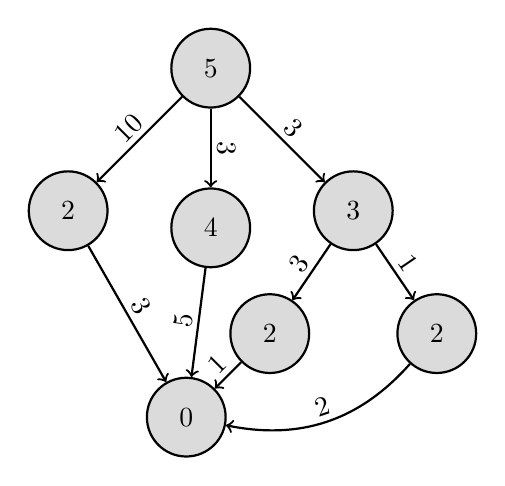
\begin{tikzpicture}[node distance={15mm}, thick, main/.style = {draw, circle,minimum size=10mm,fill={rgb:black,0.5;white,3}}, el/.style = {inner sep=2pt, align=left, sloped},
every label/.append style = {font=\tiny}] 
\centering
\node[main] (1) {$5$}; 
\node[main] (2) [below right of = 1, xshift = 7.5mm, yshift = -7.5mm] {$3$}; 
\node[main] (3) [below left of =1, xshift = -7.5mm, yshift = -7.5mm] {$2$}; 
\node[main] (5) [below =of 1, yshift = 5mm] {$4$}; 
\node[main] (4) [below right of = 2, yshift = -5mm] {$2$};
\node[main] (6) [below left of = 2, yshift = -5mm] {$2$}; 
\node[main] (7) [below left of=6] {$0$}; 

\path[->]
(1) edge node[el, above] {3} (2)
(1) edge node[el, above] {10} (3)
(1) edge node[el, above] {3} (5)
(2) edge node[el, above] {1} (4)
(2) edge node[el, above] {3} (6)
(5) edge node[el, above] {5} (7)
(3) edge node[el, above] {3} (7)
(4) edge[bend left] node[el, above]{2} (7)
(6) edge node[el, above] {1} (7)
; 
\end{tikzpicture} 
\caption{Example graph. Distance is represented on the edges. The heuristic value is represented in the node.}
\label{fig: heuristic graph}
\end{figure}

When we use the greedy algorithm in this example, it will select the worst possible route with a path cost of 13. This is because it believes the first node it chooses, with a heuristic of 2, is the closest to the goal and therefore must have the shortest path cost. 

This search is a form of pathfinding. More often than not, one would want a more accurate algorithm in order to find the most optimal path, however, in cases where there are not many obstacles, a greedy search can prove to be just as good, with the added benefit of having to do fewer computations making it easier to implement. This is why someone may choose this algorithm over a more optimal one, such as the A* search.

\textbf{A* search}

The A* algorithm takes both path cost and our chosen heuristic into consideration. The evaluation function for an A* search is $f(n) = g(n) + h(n)$. Given this, we can see how the issue we had with our greedy search is overcome. The steps of an A* algorithm are identical to the steps of a Uniform-Cost search, only we use $g + h$ instead of only $g$. One of the main issues with a UCS is that it explores paths very far off course from our goal, the A* method combats this. If we were to apply the A* algorithm to the example graph in figure \ref{fig: heuristic graph}, we would get a path cost of 6, which is the best possible path. 

\subsubsection{\Large{Adversarial search}}

In section \ref{Agents and Environments} we talked about multi-agent scenarios and how they can work together, however, what happens when they work against each other? Each agent must now consider the actions other agents could take and how these actions could affect them. These are now adversarial search problems, otherwise known as games. Our environment is now a competitive one. 

In order to solve multi-agent competitive scenarios (adversarial search problems) we can use game theory. Mathematical game theory analyses strategies in competitive situations where the outcome of a participant's choice of action depends critically on the actions of other participants. In our case, the actions of one agent will depend on the actions of another. 

To determine how to solve our problem, we first need to define it. A game can be defined as a search problem if it has the following:

\begin{itemize}
    \item Initial state - How the game is set up.
    \item Player(s) - Which player has the move in a state?
    \item Actions(s) - Possible moves in a state, s.
    \item Result(s, a) - the result of action a in state s.
    \item Terminal-Test - True when the game is over, otherwise false.
    \item Utility(s, p) - The utility function defines the final numeric value of the game. For example, in chess, you have 1 for a win or 0 for lose. A zero-sum game is one where the payoff to all players is the same every game, i.e. in chess either 1 \& 0 for win/lose or 0.5 \& 0.5 for a draw.
\end{itemize}

This helps us begin our game tree. A game tree in MinMax uses the initial state, actions and results as defined in our search problem. For example, take a look at the example game tree in \ref{fig:game tree example} 

\begin{figure}[!htp]
    \centering
    \includegraphics[width=0.8\textwidth]{Dissertation/Pictures/game tree example.png}
    \caption{Tic-tac-toe game tree example \cite{russell2016artificial}}
    \label{fig:game tree example}
\end{figure}

Here we can see the first branch is all the possible moves of player 1, followed by the min branch, which is all the possible moves of player 2 against all the possible moves of player 1 and so on and so on.  In order to get the most optimal actions, we need to pick the correct value at each node, an example of this can be seen in figure \ref{fig:game tree value example}.

\newpage
\begin{figure}[!htp]
    \centering
    \includegraphics[width=\textwidth]{Dissertation/Pictures/game tree example 2.png}
    \caption{Game tree values example \cite{russell2016artificial}}
    \label{fig:game tree value example}
\end{figure}

Figure \ref{fig:game tree value example} shows the example of a game between 2 players with a depth level of 1. The branches from node A are the available actions of player 1, who wishes to maximise the utility. The branches from nodes B, C, and D are the actions that player 2 can take given the action of player 1. The leaves of the tree show the utility of Player 1 choosing action $a_i$ where $i$ $\in\{1, 2, 3\}$ and player 2 choosing action $X_i$, where X $\in\{ B, C, D \}$. To choose the action player 1 should take, we start from the bottom of the tree and work our way up. The first step is for player 2 to select the action that \textit{minimises} the utility for player 1. This means that at node B they choose action $b_1$, at node C they choose action $c_1$ and at node D they choose action $d_3$. We now label these nodes with these values, as shown in the figure. Next, player 1 wishes to \textit{maximise} its own utility so it chooses action $a_1$.

In order to work out the utility of a state, we need to create an evaluation function. This function should take in state and return some value. It is important that our functions return a value that correctly describes the value of a state in order to ensure that our tree is as accurate as possible. We will describe later in \ref{chapter: implementation} how we created the evaluation function for our own implementation. 

Now, this method is very good at giving us an idea of the best move to take, however, it can be very costly. In the example in \ref{fig:game tree example}, tick-tac-toe, there are 9! (362880) possibilities, but we know that some moves are not worth exploring further as we have already explored a better option. We want to \textit{prune} this brunch, computing fewer options. Let's now see how we could apply alpha-beta pruning to our example game tree in figure\ref{fig:game tree value example}.

\begin{figure}[!htp]
    \centering
    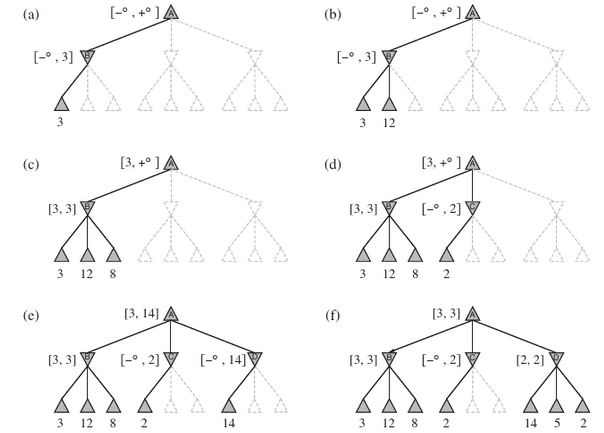
\includegraphics[width=0.8\textwidth]{Dissertation/Pictures/Pruning example.png}
    \caption{Game tree values example \cite{russell2016artificial}}
    \label{fig: pruninmg example}
\end{figure}
\newpage
In the figure \ref{fig: pruninmg example} we can see that we first explore the leftmost branch fully, then we begin to explore the next branch. The first leaf we get to in the next branch returns a value of 2. We know already that we could select the first branch ad get a result of 3, whereas no matter how far we explore the second branch, it will either return 2 or lower, due to player 2 wishing to minimise. Given this, we can prune the branch here as it is not worth exploring further, and move on to the next. The next branch first returns a value of 14. This is higher than our current max of 3, therefore we should continue to explore this branch in hopes that we can get an even higher result. now, rather than working out all 9 possible values, we have only worked out 7 and still have the same result. As the depth of our tree increases, the amount of time we same will become much more useful. 

But what if our opponent doesn't play optimally? We could've made a better move but we didn't because we assumed the enemy would make some optimal choice. What if we take a chance? This is the \textbf{Expectimax} algorithm. The Expectimax algorithm works by taking a chance on an action that we previously may not have chosen. We take a look at the values returned by our evaluation function, sum them up and divide them by the probability that we pick this path. In most cases, this is 1/$b$, where $b$ is the number of branches/moves we can take. We can apply the Expectimax algorithm to the game in figure \ref{fig:game tree value example}
\newpage
\begin{figure}[!htp]
    \centering
    \includegraphics[width=0.7\textwidth]{Dissertation/Pictures/expectimax example.png}
    \caption{Expectimax values example}
    \label{fig: expectimax example}
\end{figure}

The new values show how we explore our tree. In this example, we still choose the same move as before, going down $a_1$, but we had the opportunity to pick a different route if its new score was higher. This is a good algorithm to use when our opponent does not play optimally as it gives us the opportunity to gain extra utility. The downside of the Expectimax algorithm is that it is not optimal. This means that if our opponent does play optimally, we could lose out on points and even potentially lose the game. There is also no pruning involved in this method meaning that we have to explore the whole game tree. 

\subsection{Reinforcement Learning}\label{Reinforcement Learning}

The last idea we will introduce is reinforcement learning. Reinforcement learning is a form of machine learning which allows an agent to use trial and error to learn using its own experience. The basic idea:

\begin{figure}[!htp]
    \centering
    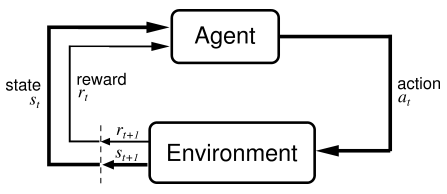
\includegraphics[width=0.7\textwidth]{Dissertation/Pictures/reinforcement learning agent.png}
    \caption{The agent-environment interaction in reinforcement learning\cite{The-Agent-Environment-Interface}}
    \label{fig: reinforcement-learning-model}
\end{figure}

An agent chooses some action, $a_1$, and receives feedback in the form of a reward $r_1$, given by some defined reward function, similar to the evaluation function for our MinMax search in \ref{Search Algortithms}. The agent must learn how to maximise its rewards. 

We have some key elements in reinforcement learning:
\begin{itemize}
    \item A policy which maps states to actions.
    \item A reward signal - each state has a value and we want to maximise the sum of the states we visit. 
    \item A value function specifies what is good in the long run.  The value of a state is the total amount of reward the agent can accumulate if it starts from that state (Kostas Stathis 2022).
    \item A model allows the agent to make inferences on how the environment will behave.
\end{itemize}

There are different forms of reinforcement learning that can be used. We will be implementing \textbf{Q-Learning}, an off-policy approach to finding the optimal value function. It is off-policy because an action is selected greedily and not according to a specific policy. We use Temporal Difference Learning to update a table in Q-Learning. A simple TD update rule can be given as:

\counterwithout{equation}{chapter}
\begin{equation}\label{eq:1}
    V(S_t) \xleftarrow{} V(S_t) + \alpha[R_{t+1} + \gamma V(S_{t+1}) - V(S_t)]
\end{equation}

Let's break down the equation \ref{eq:1} so we can understand it better. First, $V(S_t)$ is our current estimate of the state $S_t$ given by our value function. To update this we have:
\begin{center}
    (current value of the state)  $\xleftarrow{}$ (current value of the state) + $\alpha$[(reward of the new state) + $\gamma$(value of the new state) - (value of the current state)]
\end{center}
\begin{itemize}
    \item $\alpha$ is a hyper-parameter $\alpha \in$ [0, 1], representing the learning rate.
    \item $\gamma$ is a hyper-parameter $\gamma \in$ [0, 1], representing the discount rate.
    \begin{itemize}
        \item We will discuss what these hyper-parameters do in more detail.
    \end{itemize}
\end{itemize}

Making use of the Temporal Difference update rule, we can use tabular Q-Learning and come up with a new equation, given as:
\begin{equation}\label{eq:2}
    Q(S_t, A_t) \xleftarrow{} Q(S_t, A_t) + \alpha[R_{t+1} + \gamma \max_{a \in A} Q(S_{t+1}, a) - Q(S_t, A_t)
    ]
\end{equation}

Here, $Q(S_t, A_t)$ is our state $S$ given action $A$ at time $t$. Rather than having  $\gamma V(S_{t+1})$ as we did in equation \ref{eq:1} we choose the maximum action we could take given the current state.

We use three hyper-parameters in this algorithm. A hyper-parameter is a parameter whose value is used to control the learning process. We have already seen two of them, $\alpha$ and $\gamma$, the last is $\epsilon$. In reinforcement learning, we need to find a balance between exploration and exploitation. An agent will want to exploit - take actions it has tried in the past and knows to be effective. But in order to exploit, it has to have explored to find the value an action has and to make better choices in the future. To do this, we use $\epsilon$. We set $\epsilon$ to some value, between 0 and 1. Before we choose an action, we randomly generate a number between 0 and 1. If the number we generated is lower than $\epsilon$, we choose to \textbf{explore}, and given the current state, randomly pick our next action. If our random number is larger than $\epsilon$ then we choose to \textbf{exploit} and choose the action with the highest reward, as stored in our table. The higher we set $\epsilon$ to be, the more likely we are to explore, and the lower we set it the more likely we are to exploit. We can experiment with this value to find the best parameter. 

There are two types of environments in RL, episodic and continuous. A continuous environment is one that continues indefinitely such as a robot with a long life span. An episodic environment has a terminal state and therefore can be split into episodes. In our case, we will be traversing a maze in order to find some goal, which will be our termination state. Each time our agent finds the goal we start a new episode, updating the table and hopefully getting more accurate (learning) from each episode. Because we are in an episodic environment, we can change the value of $\epsilon$ every episode to make it slightly smaller and therefore choose to exploit more often each episode, i.e learning to choose the best action. 

The next hyper-parameter we will look at is $\gamma$. We use $\gamma$ to determine whether we care more about future rewards or immediate rewards. Our return in the long run can be written as:
\begin{equation}
    G_t = R_{t+1} + R_{t+2} + ... + R_T
\end{equation}

Where $R_{t+1}$ is the sequence of rewards received after time $t$, and $T$ is the final time step (Kostas Stathis 2022). When we introduce the discount factor this becomes: 
\begin{equation}
    G_t = R_{t+1} + \gamma R_{t+2} + \gamma^2 R_{t+3} + ... = \sum_{t=0}^{\infty} \gamma^t R_{t+1}
\end{equation}

We can see that if we set $\gamma$ very low, say the extreme of 0, then we only care about immediate reward, $R_{t+1}$, but as we increase $\gamma$ now the reward at $t$ worth $\gamma^{t-1}$ times what it would be if received immediately. $\gamma$ usually ranges from 0.5-0.99, but is domain-dependent, we can experiment with different values and see how this changes the behaviour of our agent.

The last hyper-parameter we have is $\alpha$, the learning rate, sometimes called step size, and $\alpha \in [0, 1]$. A determines how much we \textit{learn} from each update. If $\alpha$ is very low, then the impact it has on the table is very little and we don't learn much from the action, however, if it is too high then the updates will be greatly affected by short-term noise \cite{nian2020review}. We can tune this parameter by testing out different values and seeing the impact it has on the agent's behaviour.  

We will implement reinforcement learning to train an agent to find the goal in a maze as quickly as possible. We will perform experiments with different $\alpha$ and $\gamma$ values to see which values work best for our agent.

\chapter{Implementation}\label{chapter: implementation}
\section{Maze}\label{Maze implementation}

The first step for implementation is to design a maze. In order to generate the maze randomly some research was done about maze generation. A useful tutorial\cite{maze} which explained how to generate a perfect maze (a maze with no cycles) was used to help get started. Once this implementation was understood, it was used as the base for the maze generation. After generating a few random mazes, there was a realisation that it would be difficult to get fair experiment results with different algorithms if they were not able to be applied to identical mazes. To fix this issue, the generated mazes were saved as two-dimensional arrays so that they could then be reloaded and reused. To do this we created a maze object. The maze object takes the requested dimensions of the maze as parameters, and a two-dimensional array; this way, a new maze is only generated if the maze parameter is empty, otherwise, it loads the saved maze.

\begin{figure}[h]
     \centering
     \begin{subfigure}[h]{0.3\textwidth}
         \centering
         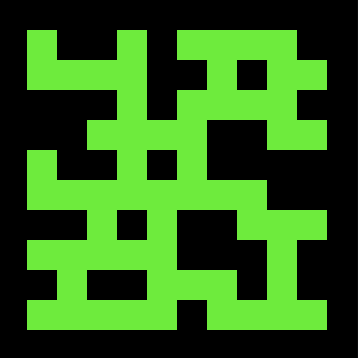
\includegraphics[width=1\textwidth]{Dissertation/Pictures/small.png}
         \caption{Small: 12 x 12}
     \end{subfigure}
     \hfill
     \begin{subfigure}[h]{0.3\textwidth}
         \centering
         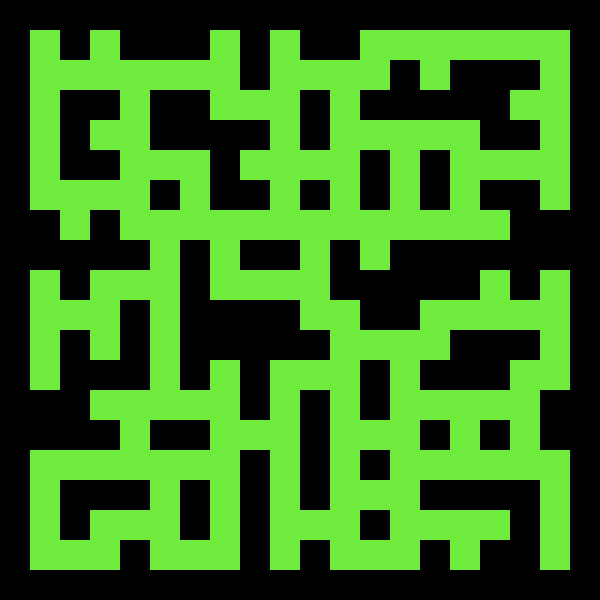
\includegraphics[width=1\textwidth]{Dissertation/Pictures/Medium.png}         
         \caption{Medium: 20 x 20}
     \end{subfigure}
     \hfill
     \begin{subfigure}[h]{0.3\textwidth}
         \centering
         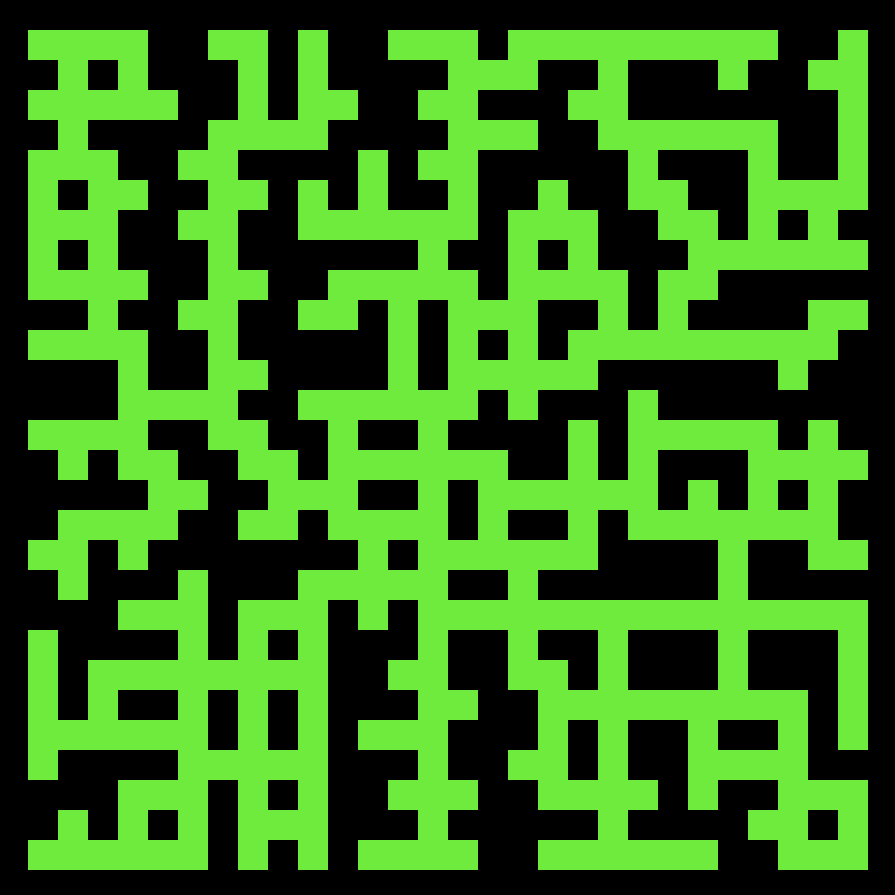
\includegraphics[width=1\textwidth]{Dissertation/Pictures/large.png}
         \caption{Large: 30 x 30}
     \end{subfigure}
     \caption{Maze generation}
     \label{fig: original mazes}
\end{figure}

The smallest maze we have is 12 x 12 cells. Originally the idea was to have the maze sizes go up in tens, however by having a maze size of 10 x 10 there were only 1-2 cycles at most. It was decided that a maze with more cycles would be a better way to showcase the algorithms abilities, so the dimensions were changed to 12 x 12. The largest maze is 30 x 30. These dimensions are large enough to showcase the agent and algorithms without wasting time repeating similar actions on a large scale.

The mazes are stored in 2D arrays, each element representing a row in the maze. This means when selecting a location on the maze, say for a goal, it has to be in the form (y, x). Storing the maze in this way is more understandable when working with the code from a programmer's perspective.

The goal of this project is to display how an agent behaves whilst trying to achieve some goal so this reason representation of agents and goals was made to be very simple. An agent in the maze is represented by a blue square. Goals are represented with a red square.

In order to model the maze as a search problem, we have a class to turn the maze into a graph representation. An attempt was made to show a visualisation of the maze using networkx and matplotlib (python libraries), however, it didn't appear helpful, see appendix \ref{Graph visualisation} for more details. The graph is represented as a dictionary with the 2D-array coordinate as the key, the value being an array containing each child, the distance to the child and the steps to reach the child. It was important to add the steps to reach the child node otherwise the agent would not be able to display these steps throughout its execution of the algorithms.

A point in the maze is identified as a edge if it has exactly 2 two children. A point with exactly 2 children is simply the path taken between 2 nodes. A point with one child is a leaf node. In figure \ref{Nodes} the cells identified to be a node have been highlighted in purple.

\begin{figure}[h]
     \centering
     \begin{subfigure}[h]{0.45\textwidth}
         \centering
         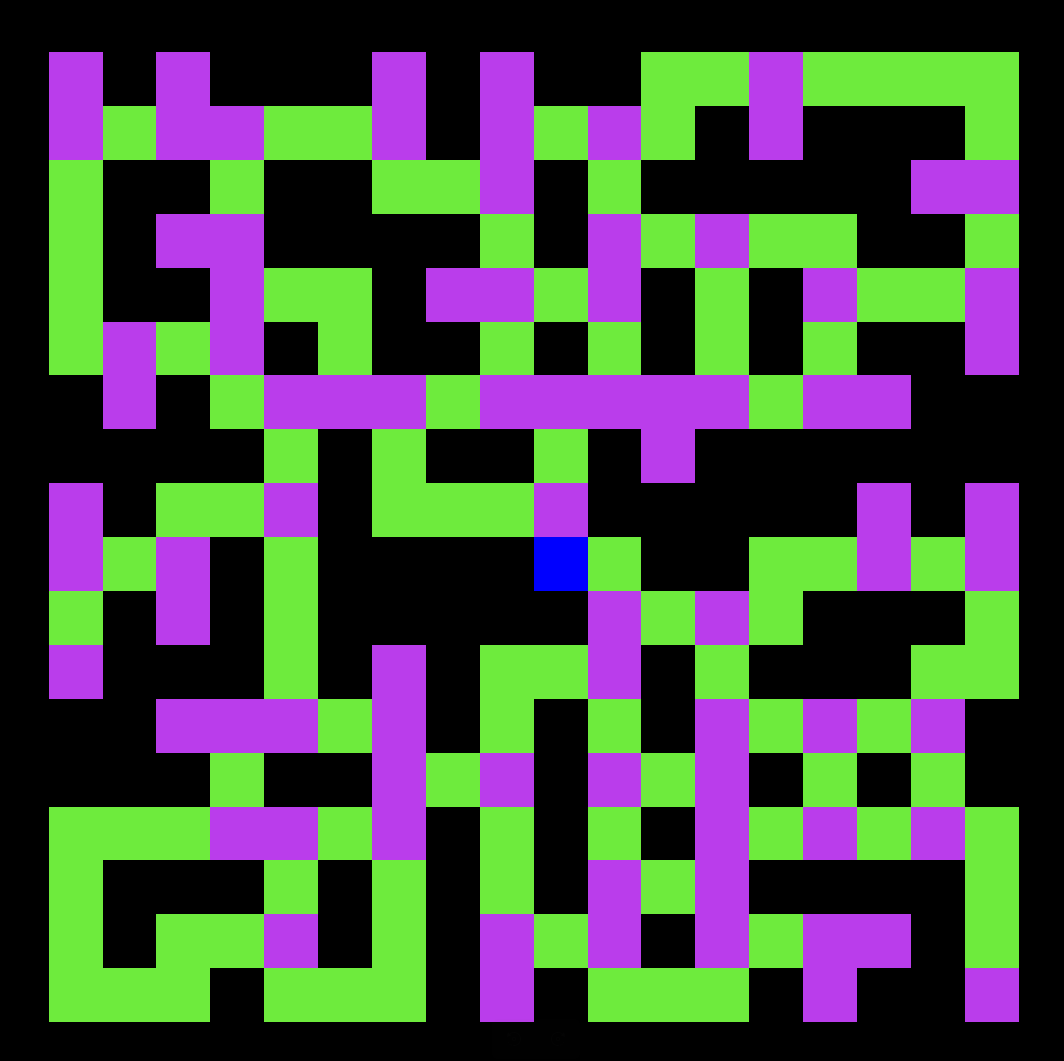
\includegraphics[width=1\textwidth]{Dissertation/Pictures/Nodes.png}
         \caption{Identified nodes on maze}
     \end{subfigure}
     \hfill
     \begin{subfigure}[h]{0.45\textwidth}
         \centering
         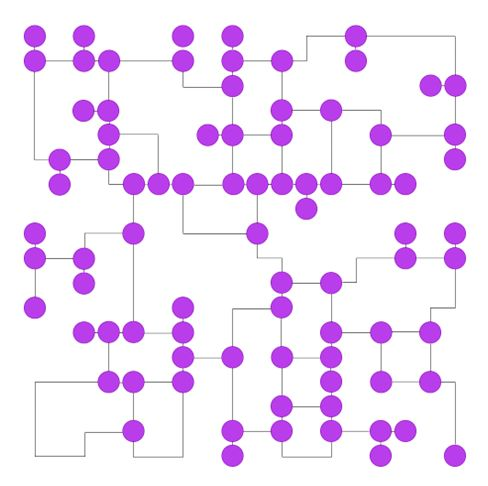
\includegraphics[width=1\textwidth]{Dissertation/Pictures/Graph.jpeg}
         \caption{Graph representation}
     \end{subfigure}
     \caption{Nodes within maze}
     \label{Nodes}
\end{figure}

\textbf{Maze changes}

Later on during the project, we needed to add multiple agents to the maze. These agents were to behave as enemies and chase our player agent, however, this was difficult to implement on the mazes we had in \ref{fig: original mazes}. This is because the player agent was prone to be trapped into a dead end. The new mazes do not have any dead ends that our agent could get caught in. The player agent was also changed to yellow and the background to a different shade of green to make it a bit nicer for the eyes. You will also notice white circles in the maze, these represent items that our agent has to collect during play. Only once all are collected is the agent able to stop. They are the goals. 

\begin{figure}[!htp]
     \centering
     \begin{subfigure}[h]{0.3\textwidth}
         \centering
         \includegraphics[width=1\textwidth]{Dissertation/Pictures/Small-new.png}
         \caption{Small: 12 x 12}
     \end{subfigure}
     \hfill
     \begin{subfigure}[h]{0.3\textwidth}
         \centering
         \includegraphics[width=1\textwidth]{Dissertation/Pictures/Medium-new.png}         
         \caption{Medium: 20 x 20}
     \end{subfigure}
     \hfill
     \begin{subfigure}[h]{0.3\textwidth}
         \centering
         \includegraphics[width=1\textwidth]{Dissertation/Pictures/Large-new.png}
         \caption{Large: 30 x 30}
     \end{subfigure}
     \caption{Maze generation New}
\end{figure}

\newpage
\section{Algorithms}

\subsection{Uninformed Search}

Now that we have our maze, we need to write the algorithms for uninformed searches. Test Driven Development (TDD) was used when writing the uninformed searches. To do this, a library called unittest was used, which when ran from the command line informs you which tests failed or passed. A test maze was created and saved so that we were able to check that the algorithms were returning the expected values.

When implementing the UCS a priority queue was not used, that is, a priority queue class was not created and implemented into the algorithm. Instead, we use a function that returns the item with the highest priority (lowest path cost). This was done for two reasons. 
\begin{itemize}
    \item The first reason was that the graph is stored in a way that passing all the values to a priority queue seemed inefficient as they would have to be rearranged in a conflicting way to the other lists.
    \item The second reason was in creating a priority queue, we would have to create the same function in order to pop the item with the highest priority, therefore by not explicitly creating a class priority queue, we could be more efficient with my time.
\end{itemize}

\subsection{Informed search}

\textbf{Collect all items in the maze using A* algorithm}

To create an algorithm that traverses the entire maze we use the A* algorithm to find the next closest item to collect, and then add that to a list, and then continue this until all items are in the list that can be returned to the agent as a route to follow. This worked when there were no agents, but once we start adding opponents this needed to change. When we implemented a reflex agent to solve the same problem, it calls the same function but only gets a path of a small length. This is because the enemy is able to chase the agent and therefore our agent needs to be able to react and change course accordingly. Because of this, it means that most of the route it would have worked out will now be scraped a new route will be generated. Having a small route be returned means that it's quicker, so there is less buffering from the visualisation aspect, but it also means that the agent doesn't waste time computing a route that it most likely will not finish.

\subsection{MinMax algorithm}

When implementing the MinMax Algorithm we needed to design an evaluation function for the agents. The aim is to inform the agent of the utility of the state so that it can make the best decision on which action it should take. The evaluation function is written as:

\begin{verbatim}
def evaluationFunction(self, state, enemy, past):
    score = 0
    if state == enemy:
        score = -math.inf
    elif state in self.goal and state not in past:
        score = 1000
    elif score == 0:
        dist = self.best(state)
        score = 100/dist
    if state in past[-2:]:
        score = -15
    return score
\end{verbatim}

We start with a score of 0. If the \verb|state| is the state that we are evaluating. \verb|enemy| is the position of the enemy (in the case of multiple enemies, the function will be called multiple times with each enemy). \verb|past| is the past 2 steps taken. What this function is saying is:
\begin{itemize}
    \item If this state has an enemy, do not go there.
    \item If this state has not been visited yet, meaning there is an item to collect, + 1000 points
    \item If the state is empty, the value is equal to 100/distance to the next closest item to collect
    \item Last, it penalises the agent for going back to the state they just were. This is because, without this check, the agent is prone to get stuck going back and forth between two positions. It doesn't however ban it completely as sometimes going backwards is the best option. 
\end{itemize}

This evaluation function is also used for the Expectimax agent.

In order to add pruning to the MinMax agent only one line had to be added to the min function. We have a check, stating that if the current score is less than a branch we have already explored, then stop checking down this branch as we already have an item which is higher therefore we know we would pick that branch over our current one so we can stop. 

In the final deliverable, the option of the MinMax algorithm \textit{without} pruning will not be available. This is because as we increase the depth it gets very slow and therefore is not worth displaying, especially since the outcome would be identical to that with pruning in terms of steps taken. 

We did not run any tests on the adversarial searches as the results would be similar to those we have already seen, however if anyone would like to compare run time and path length they can do so given the final deliverable.

\subsection{Reinforcement Q-Learning}

When implementing tabular q-learning, we used a dictionary where the key is a state and the value is a list of length 4, representing actions \textit{left, right, up, down}, in that order. Initially, the scores we all set to -1, this incentivizes the agent to move around compared to if they were initially set to 0. 

For every new episode, the epsilon value is multiplied by 0.99 so that the agent exploits more over time, giving the impression that it is learning. The $\alpha$ and $\gamma$ values have been selected in the final deliverable from tests ran, they can be seen in \ref{Reinforcement Learning Experiments}. We only implemented reinforcement learning of one pre-saved maze in order to test that it works properly. Due to tine restraints we did not experiment on different mazes, however it should run with no problems if ran on other mazes. 

\section{Software Engineering}

As mentioned, TDD was used when implementing the search algorithms. TDD is a form of unit testing that forces the programmer to build from the bottom up. First, they should create a test to fail. Next, they should write just enough code for the test to pass. Then They should test again with different values. At this point, the test should fail again, and the programmer can then refactor and re-write the code so that it will pass the tests. This way the programmer is sure that this method works correctly. This is known as red-green-refactor-commit. By commit, it is assumed that the programmer is using some form of revision control system (as any good programmer should). The use of TDD was fairly difficult on this project as a lot of the testing was visual. We were able to \textit{see} that the code was being visualised correctly, but could not use TDD to test this. We could however use it on the search algorithms as we know where it should start, where it should visit next, where it should finish and how many steps it should've taken. By using TDD we were able to ensure that the algorithms were behaving correctly. 

Revision control systems are extremely useful when working on code - especially if there are multiple people working on the same project. This system allows users to checkout a version of the project in their own branch. Here, any changes made to the project will not affect any other user. Once a specific task or goal has been implemented, the user can merge back to the main branch, where everyone can now access these changes. A revision control system is also a good tool as it allows users to work on multiple devices, and means that they do not have to worry about losing the code as it is all stored online. Throughout this project, a revision control system (GitHub) was used to help keep track of work. Each new feature to be added was done in a new branch to make sure that the existing, working code wasn't messed up or lost. When a feature was completed and tested, it was merged back to the main branch. Regular commits made sure that the coed could be accessed on multiple devices, but also ensured that work wasn't lost. This is another main advantage of using a revision control system. 


\newpage
\begin{sidewaysfigure}[!htp]
    \centering
    \includegraphics[width=1\textwidth]{Dissertation/Pictures/Agent UML.png}
    \caption{UML showing Agent Inheritance}
    \label{fig:agentUML}
\end{sidewaysfigure}
\newpage
%%%%%%%%%%%%%%%%%%%%%%%%%%%%%%%%%%%%%%%%%%%%%%%%%%%%%%%%%%%%%%%%%%%%%%%%%%%%%%%%%%%%%%%
\chapter{Experiments}
\renewcommand{\arraystretch}{1}
\section{Uninformed Searches}\label{unininformed search implementation}

As seen in section \ref{Search Algortithms}, we have a few types of uninformed searches we can use when traversing through the maze. In order to test the effectiveness of each search, we ran a series of tests. Each test used a different start position and/or goal position. Each search is run 1000 times on a different, randomly generated maze each time. This way we can see the average steps taken for the algorithm to run. Each test is run on 3 different maze sizes, as seen in section \ref{Maze implementation}.

When implementing uninformed search algorithms, we need to make sure we use the correct agent. As we have a \textbf{goal} for our agent, we know it will be a type of goal-based agent. More specifically, the type of goal-based agent will be a problem-solving agent as described in \ref{Agents and Environments}. It would be possible in the case of a uniform-cost search to use a simple reflex agent. This would be a suitable option because it chooses the path of least cost at each step i.e. only cares about its current percepts, however, as the environment we are testing in will be static, it is just as efficient to use a problem-solving, goal-based agent as before.

When looking at the time complexity of our algorithms, described in section \ref{Uninformed search}, we would expect a DFS and BFS to run at roughly the same time.  As a hypothesis, we expect the UCS to do better on average than the BFS. 

\newpage
%%%%%%%%%%%%%%%%%%%%%%%%%%%%%%%%%%%%%%%%%%%%%%%%%%
\subsection{First Experiment: Goal roughly mid-way through maze}
\begin{figure}[htp!]

\captionsetup[subfigure]{format=suboverlay}
\newcommand{\subcaptionOverlay}[1]{%
  \subcaption{}%
  \begin{tikzpicture}
    \node [inner sep=0,anchor=north west]at (-10ex,3ex) (image) {#1};
    \draw node [black] {\subcapoverlay};
  \end{tikzpicture}%
}

    \centering
    \vspace{-1\baselineskip}
        \begin{subfigure}[b]{0.55\textwidth}
           \subcaptionOverlay{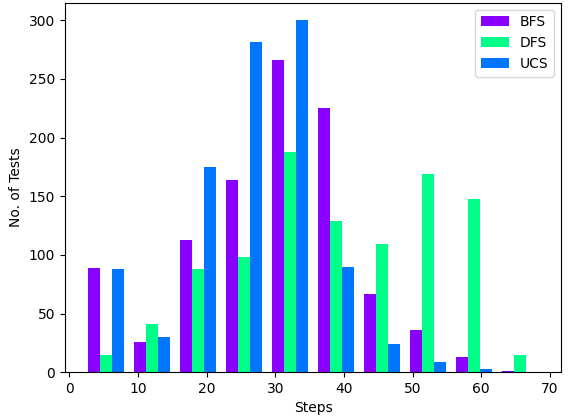
\includegraphics[width=1\linewidth]{Dissertation/Pictures/Graphs/Uninformed-mid-small.png}}
        \end{subfigure}
    \vspace{-0.1\baselineskip}
        \begin{subfigure}[b]{0.55\textwidth}
           \subcaptionOverlay{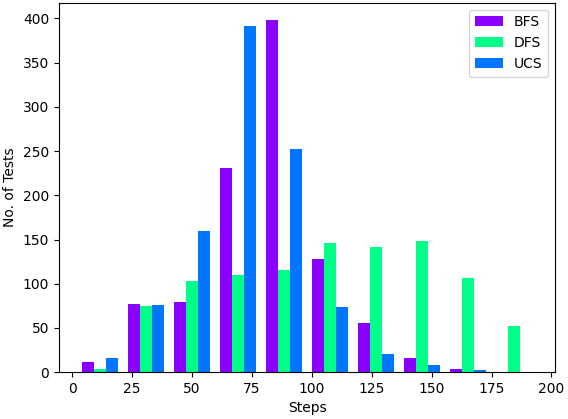
\includegraphics[width=1\linewidth]{Dissertation/Pictures/Graphs/Uninformed-mid-medium.png}}
        \end{subfigure}

        \begin{subfigure}[b]{0.55\textwidth}
        \hspace*{-0.28cm} 
           \subcaptionOverlay{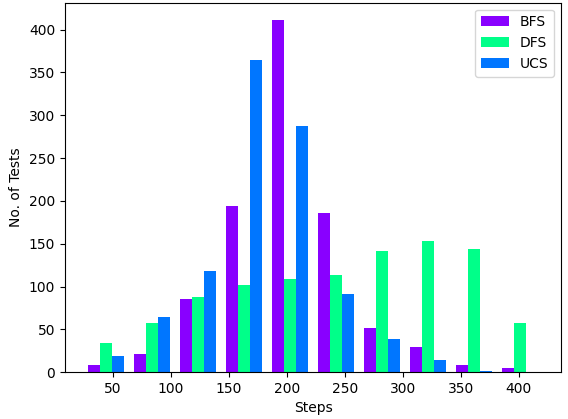
\includegraphics[width=1\linewidth]{Dissertation/Pictures/Graphs/Uninformed-mid-large.png}}
        \end{subfigure}
    \caption{Comparison of uninformed searches on mazes of different sizes. (a) A small maze. (b) A medium maze. (c) A large maze.  These graphs show the results for when the agent started in the centre of the maze to find a goal about mid-way through the maze.}
    \label{fig: Uninformed tests 1}
\end{figure}

\newpage


\begin{figure}[htp!]
\captionsetup[subfigure]{format=suboverlay}
\newcommand{\subcaptionOverlay}[1]{%
  \subcaption{}%
  \begin{tikzpicture}
    \node [inner sep=0,anchor=north west]at (-10ex,3ex) (image) {#1};
    \draw node [black] {\subcapoverlay};
  \end{tikzpicture}%
}
     \centering
     \begin{subfigure}[h]{0.3\textwidth}
         \centering
         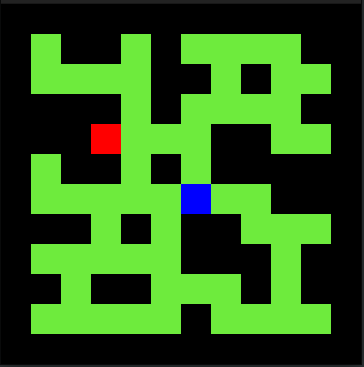
\includegraphics[width=1\textwidth]{Dissertation/Pictures/Sgoal.png}
         \caption*{Small}
     \end{subfigure}
     \hfill
     \begin{subfigure}[h]{0.3\textwidth}
         \centering
         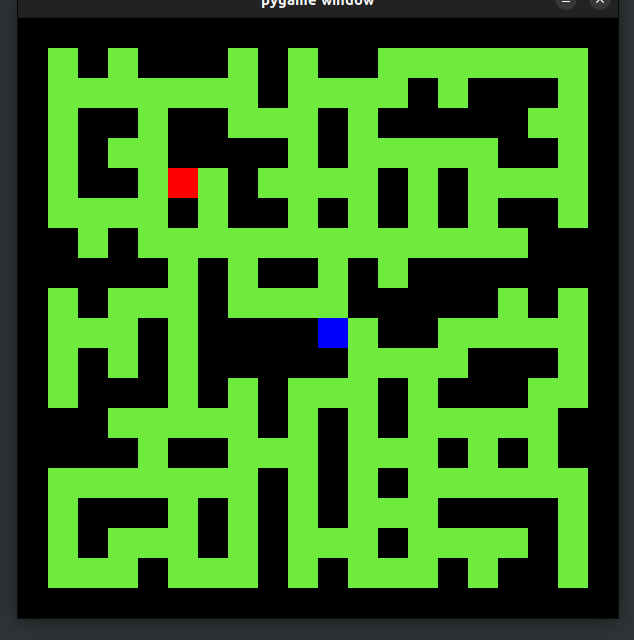
\includegraphics[width=1\textwidth]{Dissertation/Pictures/Mgoal.png}
         \caption*{Medium}
     \end{subfigure}
     \hfill
     \begin{subfigure}[h]{0.3\textwidth}
         \centering
         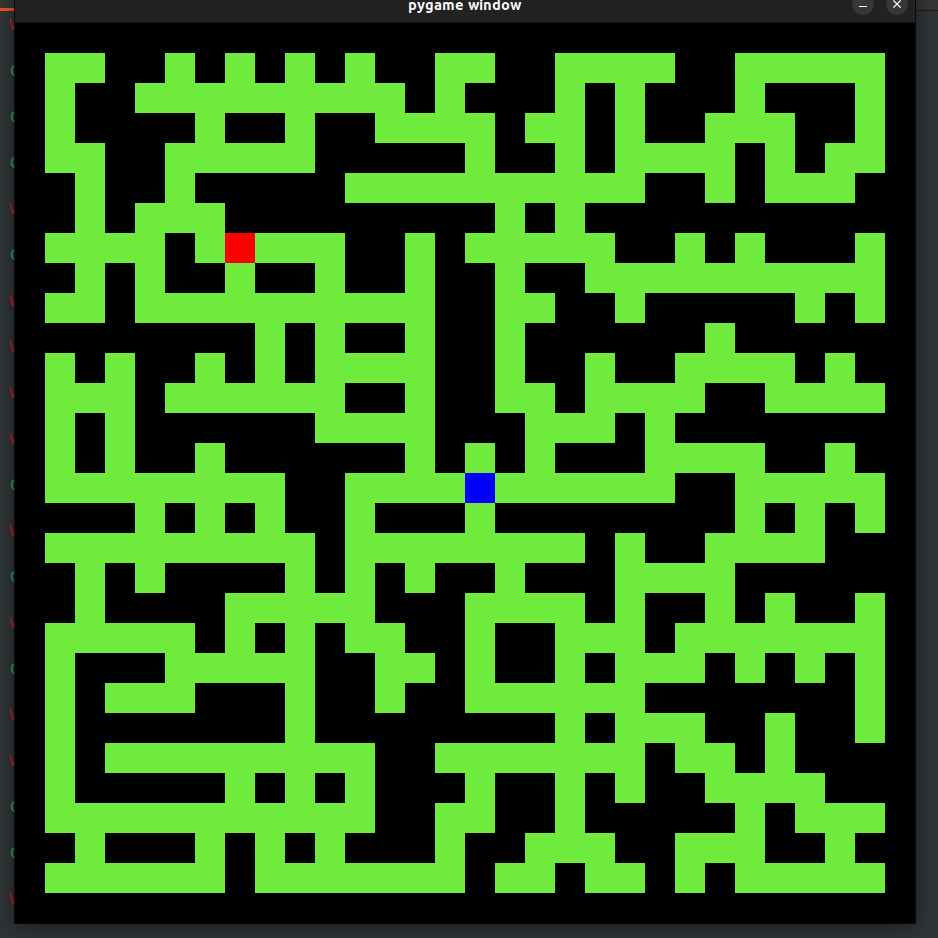
\includegraphics[width=1\textwidth]{Dissertation/Pictures/Lgoal.png}
         \caption*{Large}
     \end{subfigure}
     \captionsetup{justification=centering}
     \caption{Maze layout used in the first experiment. Goal marked with a red square. Agent marked with a blue square.}
     \label{fig: three graphs}
\end{figure}

The histograms in figure \ref{fig: Uninformed tests 1} show the number of steps taken by the agent for each test. As the maze is randomly generated it is possible that some tests had a goal either slightly closer or further from the start position, however, as the tests were run 1000 times it should give an adequate representation of the algorithm's capability. From these results we can see that each search has its own normal distribution, this is more visible when looking at results from the large maze. We can see that in all graphs the UCS does the best as it never takes the maximum number of steps, whereas the DFS has the most tests that do. On average, the BFS does better than the DFS but is not as good as the UCS. Our hypothesis that the BFS and DFS would be the same is disproved here, we can see that on average the BFS is faster. This could be because the goal was midway through meaning that the DFS likely explored down many useless paths before finding the goal.
\newpage
%%%%%%%%%%%%%%%%%%%%%%%%%%%%%%%%%%%%%%%%%%%%%%%%%%%%%%%%%%%%%%%%%%%%%%%%%%%%%%%%%%%
\subsection{Second Experiment: Goal in corner}
\begin{figure}[htp!]

\captionsetup[subfigure]{format=suboverlay}
\newcommand{\subcaptionOverlay}[1]{%
  \subcaption{}%
  \begin{tikzpicture}
    \node [inner sep=0,anchor=north west]at (-10ex,3ex) (image) {#1};
    \draw node [black] {\subcapoverlay};
  \end{tikzpicture}%
}

    \centering
    \vspace{-1\baselineskip}
        \begin{subfigure}[b]{0.65\textwidth}
           \subcaptionOverlay{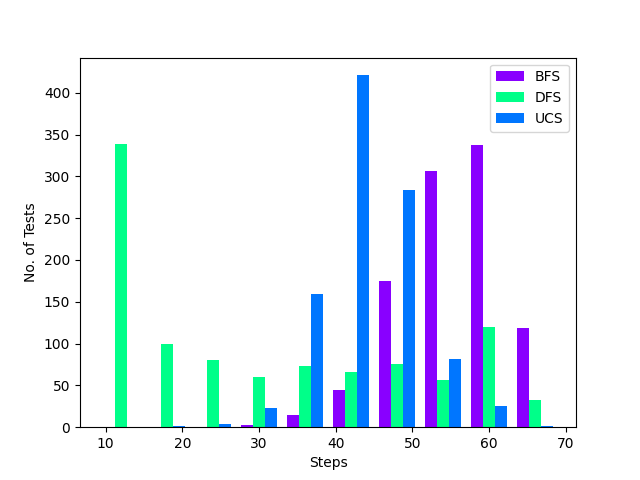
\includegraphics[width=1\linewidth]{Dissertation/Pictures/Graphs/Uninformed-corner-small.png}}
        \end{subfigure}
    \vspace{-0.1\baselineskip}
        \begin{subfigure}[b]{0.65\textwidth}
           \subcaptionOverlay{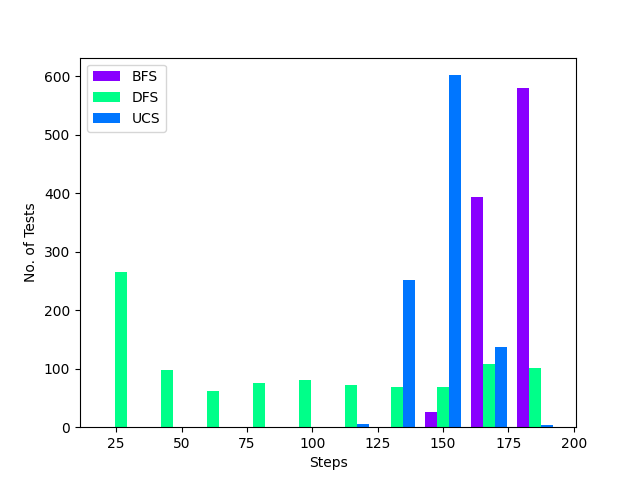
\includegraphics[width=1\linewidth]{Dissertation/Pictures/Graphs/Uninformed-corner-medium.png}}
        \end{subfigure}

        \begin{subfigure}[b]{0.65\textwidth}
        % \hspace*{-0.28cm} 
           \subcaptionOverlay{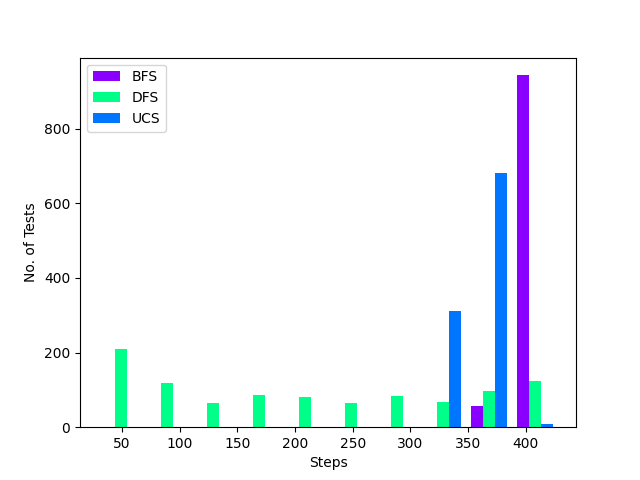
\includegraphics[width=1\linewidth]{Dissertation/Pictures/Graphs/Uninformed-corner-large.png}}
        \end{subfigure}
    \caption{Comparison of uninformed searches on mazes of different sizes. (a) A small maze. (b) A medium maze. (c) A large maze.  These graphs show the results for when the agent started in the centre of the maze to find a goal in the bottom-right-hand corner.}
    \label{fig: Uninformed tests 2}
\end{figure}

\begin{figure}[htp!]
    \centering
    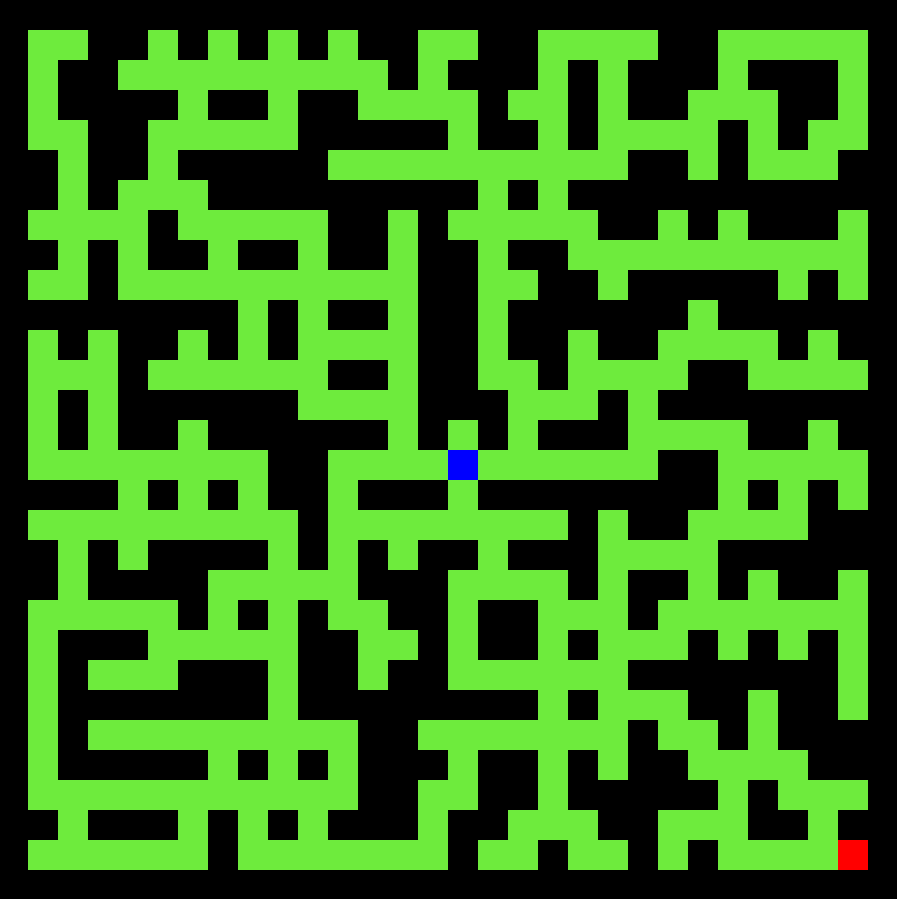
\includegraphics[width=0.5\textwidth]{Dissertation/Pictures/lCorner.png}
    \caption{Example maze used in the second experiment}
    \label{fig:my_label}
\end{figure}


We know that a DFS traverses down a single path to its end and then the next deepest and so on. This means that when our goal is in the corner, there is a chance that we find it almost instantly as a corner is one of the deepest nodes. This is visible in the graphs in figure \ref{fig: Uninformed tests 2} as we can see a high number of the DFS tests finished quicker than the other two algorithms. In its worst case, a DFS would find a corner last - however, this is also the case for a UCS and a BFS as they expand at every depth level, meaning that the corner is one of if not the last node it will visit. The graphs reflect this as we can see that the BFS takes the longest on average, with the UCS only doing slightly better, which is to be expected as it skips some edges. Like our last test this confirms our hypothesis that the UCS will do better than our BFS on average but again disproves our hypothesis that the BFS and DFS will run at roughly the same time. This is most likely because our test works in favour of the DFS whereas our last test worked in favour of the BFS.

In our next test, we will generate 1000 random mazes as before but will also generate a random goal each time. This way we can have a better feel for how our searches will do in any given scenario.
\newpage
%%%%%%%%%%%%%%%%%%%%%%%%%%%%%%%%%%%%%%%%%%%%%%%%%%%%%%%%%%%%%%%%%%%%%%%%%%%%%%%%%%%
\subsection{Last Experiment: Random goal}
\begin{figure}[htp!]

\captionsetup[subfigure]{format=suboverlay}
\newcommand{\subcaptionOverlay}[1]{%
  \subcaption{}%
  \begin{tikzpicture}
    \node [inner sep=0,anchor=north west]at (-10ex,3ex) (image) {#1};
    \draw node [black] {\subcapoverlay};
  \end{tikzpicture}%
}

    \centering
    \vspace{-1\baselineskip}
        \begin{subfigure}[h]{0.65\textwidth}
           \subcaptionOverlay{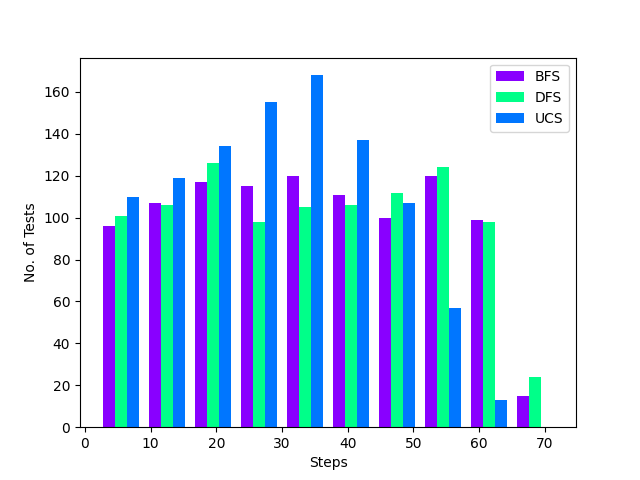
\includegraphics[width=1\linewidth]{Dissertation/Pictures/Graphs/Uninformed-random-small.png}}
        \end{subfigure}
    \vspace{-0.1\baselineskip}
        \begin{subfigure}[h]{0.65\textwidth}
           \subcaptionOverlay{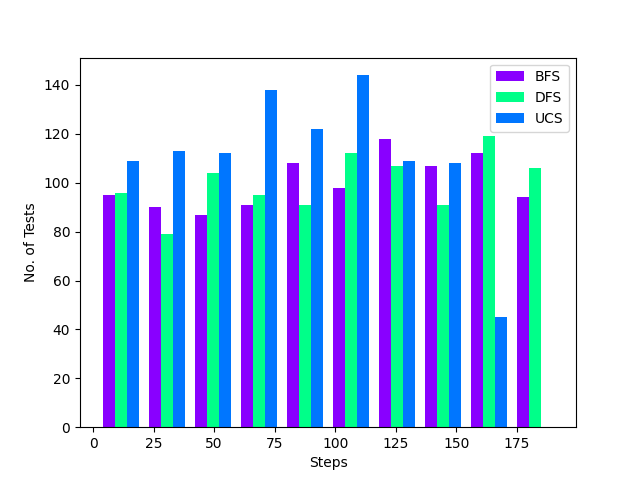
\includegraphics[width=1\linewidth]{Dissertation/Pictures/Graphs/Uninformed-random-medium.png}}
        \end{subfigure}

        \begin{subfigure}[h]{0.65\textwidth}
        % \hspace*{-0.28cm} 
           \subcaptionOverlay{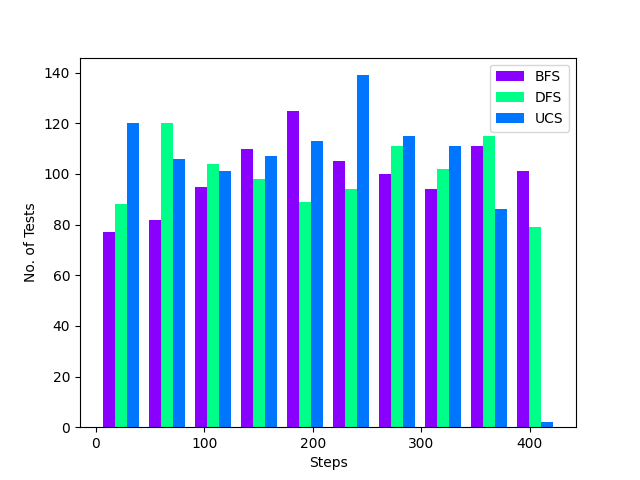
\includegraphics[width=1\linewidth]{Dissertation/Pictures/Graphs/Uninformed-random-large.png}}
        \end{subfigure}
    \caption{Comparison of uninformed searches on mazes of different sizes. (a) A small maze. (b) A medium maze. (c) A large maze.  These graphs show the results for when the agent started in the centre of the maze to find a randomly generated goal}
    \label{fig: Uninformed tests 3}
\end{figure}


In this last experiment, the agent always began in the middle, but the goal and maze were random for each test. Now we can see how each search does as a whole, with both close and far goals. When we look at the graphs in figure \ref{fig: Uninformed tests 3} we can see that both hypotheses are correct. It is clear from the absence of a blue bar at the largest number of steps in all tests that the UCS did better than the BFS on all maze sizes, making it the most optimal search out of the three. We can also see that the DFS and BFS work at roughly the same time with their results being almost identical, varying only by a few tests on the small and medium mazes.

When looking at the large maze results, it seems that the DFS was actually better than the BFS by more than a few tests, whereas the other graphs suggest they are almost equal. With this information, it suggests that when doing a search on a larger scale the DFS would actually be the most desired option.

A video of the agent's visualisation: https://youtu.be/vsaYro-G3bo

\newpage
%%%%%%%%%%%%%%%%%%%%%%%%%%%%%%%%%%%%%%%%%%%%%%%%%%
\section{Informed Searches}\label{Ininformed search implementation}

Uninformed searches work but are not efficient. Now we will use we see how we can use heuristics which give our searches information about the maze in order to make informed decisions. 

The first set of tests we will complete is deciding which heuristic is best when using an A* search to find the best route through a maze which touches all 4 corners. To do this, we will generate a random maze and test the A* with both heuristics before moving on to another maze. We will test 1000 mazes and see which heuristic is the most optimal.

\subsection{Path through the maze that touches all 4 corners}
\begin{figure}[htp!]

\captionsetup[subfigure]{format=suboverlay}
\newcommand{\subcaptionOverlay}[1]{%
  \subcaption{}%
  \begin{tikzpicture}
    \node [inner sep=0,anchor=north west]at (-10ex,3ex) (image) {#1};
    \draw node [black] {\subcapoverlay};
  \end{tikzpicture}%
}

\captionsetup[subfigure]{format=suboverlayright}
\newcommand{\subcaptionOverlayright}[1]{%
  \subcaption{}%
  \begin{tikzpicture}
    \node [inner sep=0,anchor=north west]at (-40ex,3ex) (image) {#1};
    \draw node [black] {\subcapoverlay};
  \end{tikzpicture}%
}
    \centering

        \begin{subfigure}[h]{0.4\textwidth}
           \subcaptionOverlay{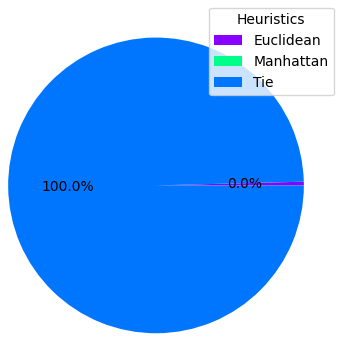
\includegraphics[width=1\linewidth]{Dissertation/Pictures/Graphs/Informed-pie-small.png}}
        \end{subfigure}

        \begin{subfigure}[h]{0.4\textwidth}
           \subcaptionOverlay{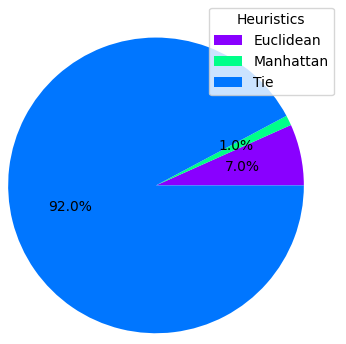
\includegraphics[width=1\linewidth]{Dissertation/Pictures/Graphs/Informed-pie-medium.png}}
        \end{subfigure}
        \begin{subfigure}[h]{0.4\textwidth}
           \subcaptionOverlayright{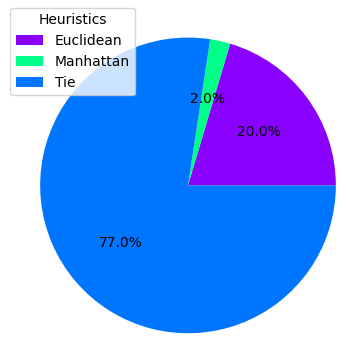
\includegraphics[width=1\linewidth]{Dissertation/Pictures/Graphs/Informed-pie-large.png}}
        \end{subfigure}
    \caption{Comparison of heuristics used in the A* algorithm on mazes of different sizes. (a) A small maze. (b) A medium maze. (c) A large maze. These graphs show the results for when the agent traversed the maze to touch all 4 corners.}
    \label{fig: informed tests 1}
\end{figure}

\newpage
\begin{figure}[!h]
    \centering
    \begin{subfigure}{0.3\textwidth}
         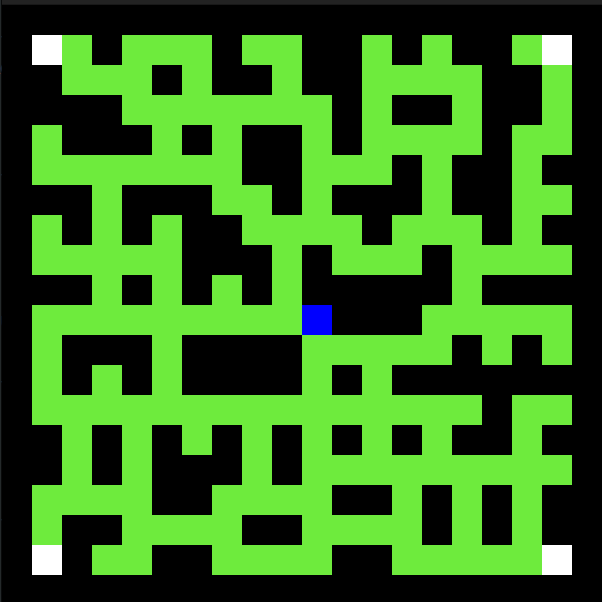
\includegraphics[width=1\textwidth]{Dissertation/Pictures/Corners-As.png}
         \caption*{Corners highlighted}
    \end{subfigure}
    \hfill
    \begin{subfigure}{0.3\textwidth}
        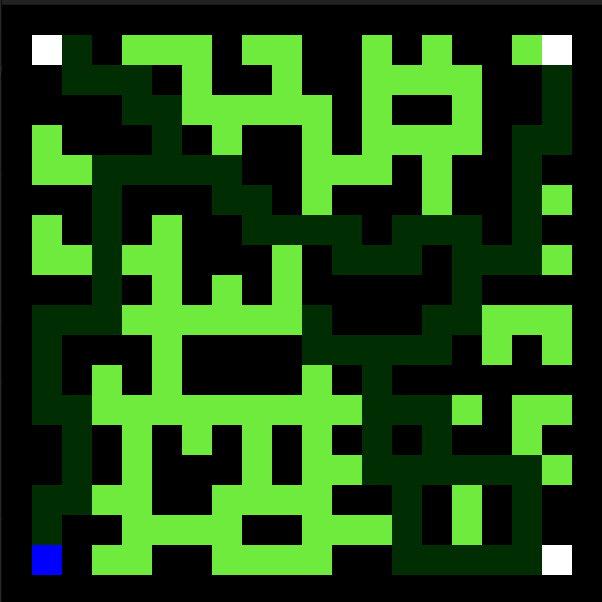
\includegraphics[width=1\textwidth]{Dissertation/Pictures/Corners-As-E.png}
        \caption*{Euclidean path}
    \end{subfigure}
    \hfill
    \begin{subfigure}{0.3\textwidth}
        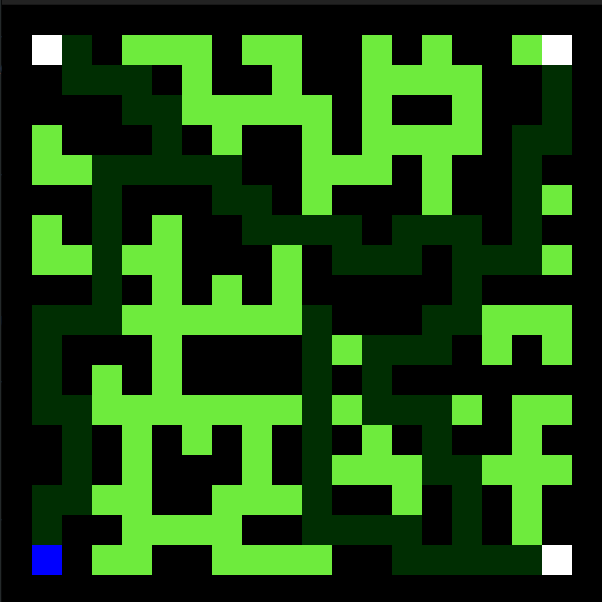
\includegraphics[width=1\textwidth]{Dissertation/Pictures/Corners-As-M.png}
        \caption*{Manhattan path}
    \end{subfigure}
\end{figure}

The pictures of the maze show an example of how the different heuristics encourage the agent to take a different path, this doesn't however guarantee any change in path distance - they could be identical. When looking at the results in figure \ref{fig: informed tests 1} we can see that when testing on a small maze the different heuristics have almost no impact, however, when we scale this up we can see that the euclidean heuristic provides a better idea for our agent, making it the fastest 20\% of the time, compared to our Manhattan which is only faster 2\% of the time. This percentage jump is fairly significant and therefore shows that the best heuristic out of the two would be euclidean. 

%%%%%%%%%%%%%%%%%%%%%%%%%%%%%%%%%%%%%%%%%%%%%%%%%%%
\subsection{Path that traverses entire maze}

 We want our agent to be able to traverse every single cell in our maze as if there were an item to collect, like in Pac-Man. We could do this one of 4 ways using our informed searches, A* and greedy. We could use the A* with the euclidean or Manhattan heuristic, or we could use our greedy with either the euclidean or Manhattan heuristic. In our last test, we found that the euclidean heuristic was more accurate on average when compared to  our Manhattan heuristic, however, we did not take into account run time. The next step is to test these 4 possibilities and see which algorithm + heuristic would be the most ideal. 

 The next three pages display the results from each maze size: small, medium and large.

\newpage
\begin{figure}[htp!]

\captionsetup[subfigure]{format=suboverlay}
\newcommand{\subcaptionOverlay}[1]{%
  \subcaption{}%
  \begin{tikzpicture}
    \node [inner sep=0,anchor=north west]at (-10ex,3ex) (image) {#1};
    \draw node [black] {\subcapoverlay};
  \end{tikzpicture}%
}

    \centering
    \vspace{-1\baselineskip}
        \begin{subfigure}[h]{0.75\textwidth}
           \subcaptionOverlay{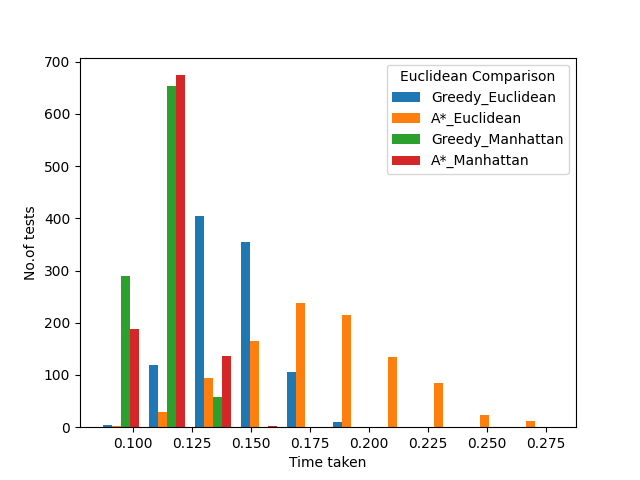
\includegraphics[width=1\linewidth]{Dissertation/Pictures/Graphs/SmallTimes.png}}
        \end{subfigure}
    \vspace{-0.1\baselineskip}
        \begin{subfigure}[h]{0.45\textwidth}
           \subcaptionOverlay{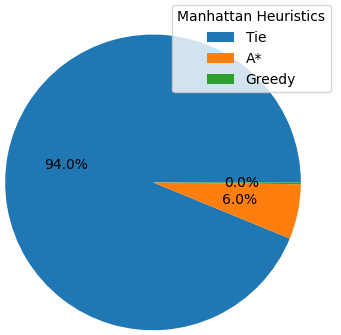
\includegraphics[width=1\linewidth]{Dissertation/Pictures/Graphs/SmallManhattan.png}}
        \end{subfigure}

        \begin{subfigure}[h]{0.45\textwidth}
        % \hspace*{-0.28cm} 
           \subcaptionOverlay{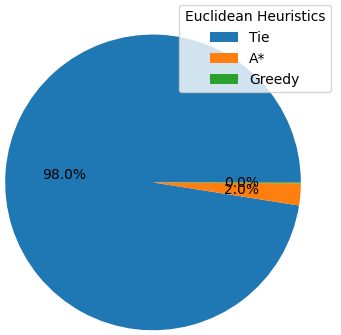
\includegraphics[width=1\linewidth]{Dissertation/Pictures/Graphs/SmallEuclidean.png}}
        \end{subfigure}
    \caption{Comparison of informed searches using different heuristics on a small maze. (a) Run time of algorithms. (b) Manhattan heuristic results. (c) Euclidean heuristic results. These graphs show the results we got after testing each informed search twice, using a different heuristic each time, to get an agent to traverse the whole maze.}
    \label{fig: informed tests 2 - small}
\end{figure}

\newpage
\begin{figure}[htp!]

\captionsetup[subfigure]{format=suboverlay}
\newcommand{\subcaptionOverlay}[1]{%
  \subcaption{}%
  \begin{tikzpicture}
    \node [inner sep=0,anchor=north west]at (-10ex,3ex) (image) {#1};
    \draw node [black] {\subcapoverlay};
  \end{tikzpicture}%
}

    \centering
    \vspace{-1\baselineskip}
        \begin{subfigure}[h]{0.75\textwidth}
           \subcaptionOverlay{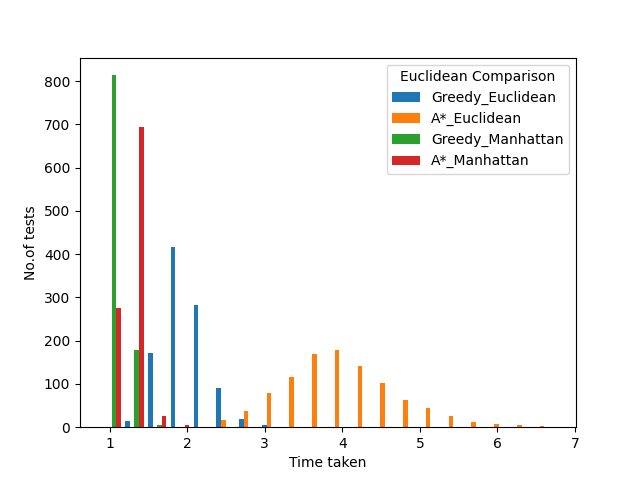
\includegraphics[width=1\linewidth]{Dissertation/Pictures/Graphs/MediumTimes.png}}
        \end{subfigure}
    \vspace{-0.1\baselineskip}
        \begin{subfigure}[h]{0.45\textwidth}
           \subcaptionOverlay{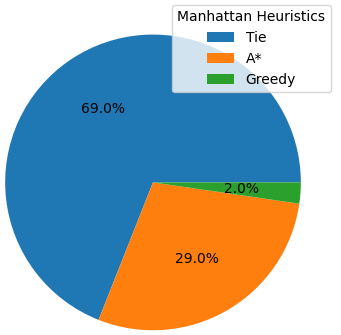
\includegraphics[width=1\linewidth]{Dissertation/Pictures/Graphs/MediumManhattan.png}}
        \end{subfigure}

        \begin{subfigure}[h]{0.45\textwidth}
        % \hspace*{-0.28cm} 
           \subcaptionOverlay{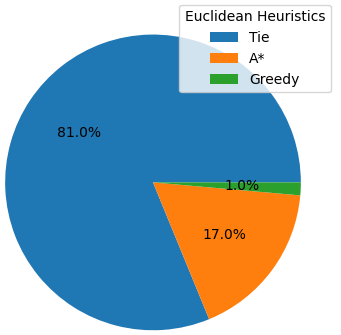
\includegraphics[width=1\linewidth]{Dissertation/Pictures/Graphs/MediumEuclidean.png}}
        \end{subfigure}
    \caption{Comparison of informed searches using different heuristics on a medium maze. (a) Run time of algorithms. (b) Manhattan heuristic results. (c) Euclidean heuristic results. These graphs show the results we got after testing each informed search twice, using a different heuristic each time, to get an agent to traverse the whole maze.}
    \label{fig: informed tests 2 - medium}
\end{figure}

\begin{figure}[htp!]

\captionsetup[subfigure]{format=suboverlay}
\newcommand{\subcaptionOverlay}[1]{%
  \subcaption{}%
  \begin{tikzpicture}
    \node [inner sep=0,anchor=north west]at (-10ex,3ex) (image) {#1};
    \draw node [black] {\subcapoverlay};
  \end{tikzpicture}%
}

    \centering
    \vspace{-1\baselineskip}
        \begin{subfigure}[h]{0.75\textwidth}
           \subcaptionOverlay{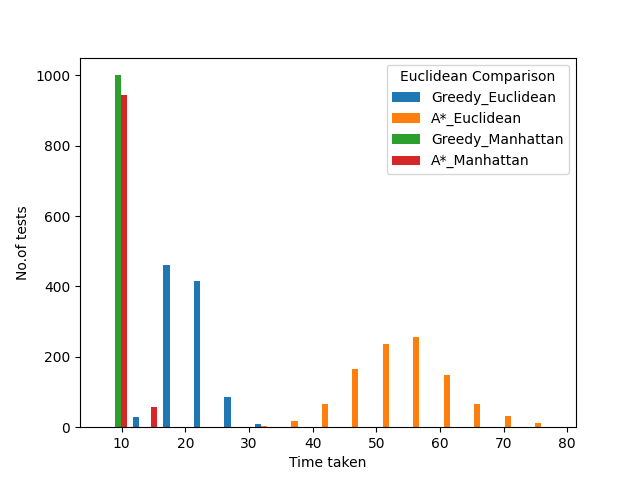
\includegraphics[width=1\linewidth]{Dissertation/Pictures/Graphs/LargeTimes.png}}
        \end{subfigure}
    \vspace{-0.1\baselineskip}
    \hspace*{-1cm} 
        \begin{subfigure}[h]{0.45\textwidth}
        
           \subcaptionOverlay{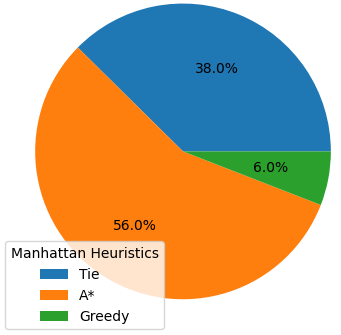
\includegraphics[width=1\linewidth]{Dissertation/Pictures/Graphs/LargeManhattan.png}}
        \end{subfigure}

        \begin{subfigure}[h]{0.45\textwidth}
           \subcaptionOverlay{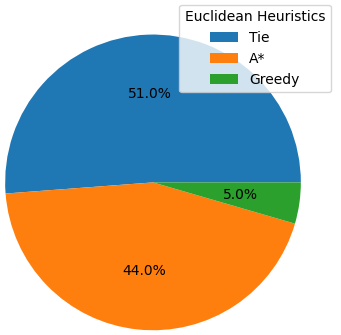
\includegraphics[width=1\linewidth]{Dissertation/Pictures/Graphs/LargeEuclidean.png}}
        \end{subfigure}
    \caption{Comparison of informed searches using different heuristics on a large maze. (a) Run time of algorithms. (b) Manhattan heuristic results. (c) Euclidean heuristic results. These graphs show the results we got after testing each informed search twice, using a different heuristic each time, to get an agent to traverse the whole maze.}
    \label{fig: informed tests 2 - large}
\end{figure}
\newpage
\textbf{Small Maze: Figure \ref{fig: informed tests 2 - small}}
The graphs in figure \ref{fig: informed tests 2 - small}, and all graphs to follow, are the results after running the algorithms 1000 times. The pie charts represent the percentage of tests that finished in the least amount of steps. We can see here that for the small mazes, the A* algorithm is always the best option, either taking the least amount of steps or drawing with the greedy algorithm. We can see from the time taken that the greedy algorithm is always fastest than that of the A* when using the same heuristic. This doesn't have a huge impact on run time, however, differing only by about 1 second.

\textbf{Medium Maze: Figure \ref{fig: informed tests 2 - medium}}
Scaling up our maze to a medium size, we can see how the search we choose begins to have a bigger impact. In figure \ref{fig: informed tests 2 - small} (b) we can see that the A* algorithm was faster by at most 6\%. This jumps to almost 5 times larger when we scale the maze up to this size, suggesting that the A* algorithm is the most desirable algorithm for this problem. We can also see that the time taken for the euclidean A* algorithm to run now takes a lot longer than the other searches, taking almost double the amount of time in some cases. This makes this variation of the A* algorithm less desirable as if we had to use it many times in one run-through, our run time would increase significantly.  

\textbf{Large Maze: Figure \ref{fig: informed tests 2 - large}}
The final set of results when ran on our large maze. We can now see that the A* is \textit{significantly} better than the greedy, taking the least amount of steps in almost half of all tests. This did however come with a price. Using the A* algorithm with the euclidean heuristic seems to be the most accurate, however, the run time has jumped massively, with the longest test taking 1.5 minutes. If this had to be computed only once it would be okay, but given that this algorithm will need to be adapted to react to other agents meaning it will have to be computed more than once, this creates a less than ideal run time. In comparison, the A* with the Manhattan is still better than the greedy, with a much more desirable run time. In fact, when comparing the results from both A* algorithms $<$1\% of the euclidean tests were faster than the Manhattan tests. 

From all of these results, it is clear that the best variation to use is the A* algorithm using the Manhattan heuristic for the most optimal path length and time taken ratio.

\newpage
\section{Reinforcement Learning} \label{Reinforcement Learning Experiments}

In reinforcement learning, we have 3 hyper-parameters, $\alpha, \gamma$ and $\epsilon$, as we saw in \ref{Reinforcement Learning}. We want to find the best values for these parameters. We ran two tests, 1 testing different values of $\gamma$, and one testing different values of $\alpha$. In all tests, we kept epsilon the same: starting at 0.4 and reducing it by 0.1\% each episode. In each test, we choose a new value for our hyper-parameter, run the code 1000 times and take the average episode length. 
\hspace*{-1cm} 
\begin{figure}[!htp]
    \centering
    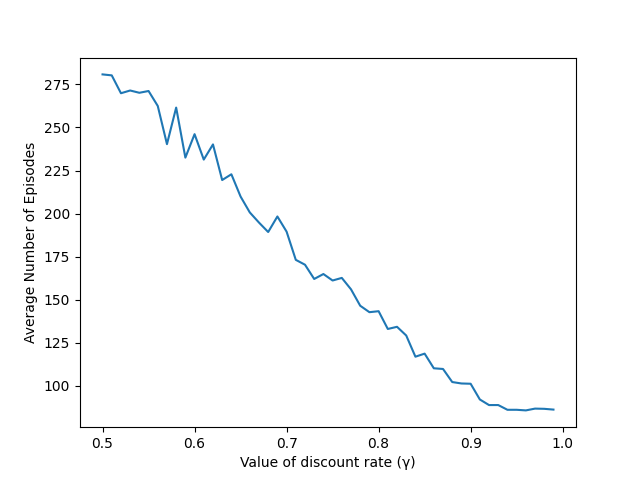
\includegraphics[width=0.7\textwidth]{Dissertation/Pictures/QLearningGamma.png}
    \caption{Increasing value of gamma, $\gamma$}
    \label{fig:gamma}
\end{figure}

We chose to only test values between 0.5-0.99 as we stated in section \ref{Reinforcement Learning} that these are the values typically used for $\gamma$. We can clearly see in figure \ref{fig:gamma} that as we increase $\gamma$, our average episode number decreases. We know that the larger we set $\gamma$ the more we care about long-term rewards. Given this scenario, it makes sense that focusing on long-term rewards over the short term gives us better results as it means our agent is focused on finding the goal node which it will not be close to when it begins. Given these results, we chose a value of 0.95 in our final deliverable.

\newpage
\begin{figure}[!htp]
    \centering
    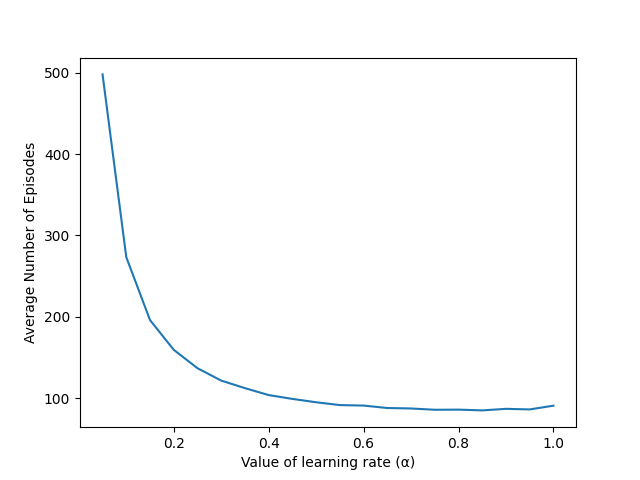
\includegraphics[width=0.7\textwidth]{Dissertation/Pictures/QLearningAlpha.png}
    \caption{Increasing value of alpha, $\alpha$}
    \label{fig:alpha}
\end{figure}

 We used a $\gamma$ value of 0.95 in these experiments. We can see in figure \ref{fig:alpha} that as we increase $\alpha$ our results because more accurate. This is drastic at first and then slows down in effect. We can see that as it approaches 1 it actually begins to increase again slightly. 

This curve can be explained. With a lower value of $\alpha$, our agent isn't learning much from its previous episodes, most likely continuing to make mistakes it should have learned from, thus having a high number of episodes, however, as we increase $\alpha$ the agent learns more about its actions meaning it finds the goal quicker  and more optimally each episode. Given these results, a $\alpha$ value of 0.8 was chosen for the final deliverable.

A video for reinforcement learning and informed searches: https://youtu.be/I2Ca1AfbSkU

\chapter{Professional Issues}  

\section{Plagiarism}

Plagiarism is the act of taking someone else's work or ideas and trying to pass them off as your own. As mentioned in section \ref{Maze implementation}, code from the website \cite{maze} was used to help write the base for the maze generation. This could be seen as plagiarism as it is being used in our project. The author and website have been referenced to ensure this won't be the case. The code has also been changed and edited in a way that fits our needs, it is not purely copied and pasted. It is also possible that some of the background theory could be seen as plagiarism as it has been used as research to help write about the main concepts. Wherever someone else's knowledge was used to help explain a concept, they have been cited.

\section{Agents}

There are a few issues that come with the use of agents. One issue that is not always thought about is the emotional connection people can develop. It is not unheard of for humans to anthropomorphise agents, which doesn't necessarily cause issues outright, but occasionally these emotions towards agents can be that of fear or resentment. Agents are commonly used to relieve users of responsibilities that the agents can handle. This can upset some users, feeling as if the agents are taking their jobs and begin to resent their use, which can affect the work environment.

Agents can also influence decision-making. In some situations, a user might not have access to the algorithm's performance and therefore follow an agent's recommendations. These algorithms can be designed to be persuasive or deceptive, leading users to make less-than-ideal choices. Agents are made autonomous with the hopes that they make choices with their goal in mind, but these goals may differ from that of the user \cite{seeber2020collaborating}.

Agents can be robotic. For example, self-driving cars or human-like robots. If one of the agents is to hurt a person, on purpose or by accident, someone has to take responsibility.  It is possible to blame the programmer, they implemented the rules that the agent has to follow; it could also be the company owner, they should've tested more thoroughly to make sure an incident like this couldn't happen.

An example of an incident involving AI is the Tesla crash in November 2022. Tesla Cars have the option of including  ``Full Self-Driving" (FSD) software. This is not included in all cars but is heavily promoted by the CEO Elon Musk. The crash occurred whilst the vehicle was in ``full self-driving mode" and resulted in two juveniles being transported to the hospital, as well as causing lengthy delays on the San Francisco Bay bridge\cite{Tesla}.

The vehicle was travelling at 55mph when the software malfunctioned, causing the car to brake suddenly, reducing its speed to 20mph. This abrupt stop led to a vehicle hitting the Tesla, then setting off a chain reaction of crashes. Tesla has stated that the cars are not autonomous and do require active driver supervision, they have also been warned that if they choose to install FSD it ``may do the wrong thing at the worst time".

In this instance, it is hard to say who is at fault. True, the driver should've been active at the wheel and therefore attempted to prevent the cash, but likewise allowing users to install software that puts the car in ``full self-driving mode" gives the impression that the car is capable of driving without the need of full supervision.

 With technology forever developing, there is often a debate on whether or not AI could be recognised as a separate legal entity existing independently of another or an organizational unit without legal personality \cite{nowik2021electronic}. This refers only to self-aware AI. If this were to happen, AI wouldn't count as material owned by a company but rather as a kind of shareholder or maybe even a person on a board of directors. We would then need to consider to what extent the owner of the AI should be responsible. Most labour laws are in place to protect the employee from unfair and unsafe work environments. By making AI its own legal identity, their laws would have to be changed/adapted to work for AI as most rules wouldn't apply, such as working hours.

%%%% ADD YOUR BIBLIOGRAPHY HERE
\newpage
\addcontentsline{toc}{chapter}{Bibliography}
\bibliographystyle{plain} % We choose the "plain" reference style
\bibliography{references} % Entries are in the references.bib file

\label{endpage}

\newpage

%TC:ignore 
\begin{appendices}
\chapter{Graph Visualisation}\label{Graph visualisation}
\begin{figure}[h]
     \caption{Graph Representation of maze}
     \centering
     \begin{subfigure}[h]{1\textwidth}
         \centering
         \includegraphics[width=0.6\textwidth]{Dissertation/Pictures/graph_fail1.png}
         \caption{Small Maze Graph}
         \label{fig: Small Maze graph}
     \end{subfigure}
     \hfill
     \begin{subfigure}[h]{1\textwidth}
         \centering
         \includegraphics[width=0.8\textwidth]{Dissertation/Pictures/graph_fail2.png}
         \caption{Large Maze}
         \label{fig: Large Maze Graph}
     \end{subfigure}
\end{figure}

I attempted to use the python libraries matplotlib and networkx to represent the nodes in the maze as a graph, however, I quickly realised this was a bad idea. Although the figure \ref{fig: Small Maze graph} is somewhat readable it is not very clear which nodes connect to each other due to the overlapping edges. To see if this was fixable I did some research, after not finding a solution and given this is not a vital piece of material, I decided to leave it out. It seems that the visualisation of the large maze in figure \ref{fig: Large Maze Graph} would be complex to read regardless given the size.
\end{appendices}
%TC:endignore 
\end{document}

\end{article}


